\documentclass[paper={210mm,297mm},line_length=35zw,number_of_lines=31,head_space=30mm,gutter=40mm,baselineskip=2.0zw,headfoot_verticalposition=1.5zw]{jlreq} %gutterを含んだレイアウトは要調整
\usepackage{luatexja}
\usepackage{graphicx}
\usepackage{float}

\begin{document}

\tableofcontents
\newpage

\section{はじめに}

\subsection{研究の背景}

2020年から現在に至るまで新型コロナウイルス感染症(以下,コロナとする)は流行している。
初期の頃は,感染力が高い上,重症化になりやすく,最悪死に至る危険性があった。
そのため,世界各国が自国民への感染を抑制するため,外出禁止や入国規制などを行った。
日本も例外ではなく,「緊急事態宣言」や「まん延防止等重点措置」など,国民に対し協力という形で感染対策に臨んだ。
しかし,感染症は拡大し,人々は新しい生活様式に努めなければならなかった。
その過程の中で,不要不急の外出の自粛や3密(密集,密接,密閉)の回避,テレワーク・在宅勤務の推奨など,従来の生活様式には無かったことを実践した。
このように,社会経済的な活動への影響は明白であり,それらを研究することは重要である。
また,現在進行形のポストコロナ社会を捉える上でも必要となる。\\
 日本におけるこれまでのコロナに関する研究の多くは,主に医療・看護・公衆衛生分野の研究である。
しかしながら,日常生活に与えた影響についての研究も存在する。
例えば,小田中・牛膓(2023)は,コロナ禍中で経験したことや対人関係の変化についてインタビュー調査を行い,その結果と既存の社会理論との関連性を明らかにしている。
また,大森・熊越(2022)は,東京都市圏の公示地価の増減と付与されている不動産鑑定士のコメントを分析し,コロナ禍で高まったニーズについて明らかにした。\\
 他方,学術研究だけでなく,政府機関の調査も行われた。
例えば,内閣府のワーキングペーパーでは,令和3年度社会生活基本調査を用いて,在宅勤務・テレワークが生活に与えた影響について分析し,男女間での差や子供の有無で生活時間に違いがあることを明らかにしている(山地ほか,2024)。
また,宿泊旅行統計調査のデータを基に,2020年における日本人及び外国人観光客の宿泊需要についての分析も行われた(栗原ほか,2022)。\\
 コロナが日常生活に与えた影響の研究は,上記のように成されているが,その多くは社会学的視点によるものだ。
他方,コロナに関する地理学的な視点の研究も存在している。
加藤(2022)は携帯電話位置情報を用いて,郊外都市における感染者数と行動範囲の相関関係を分析し,感染者数の減少と行動範囲の縮小の相関関係は低いことを明らかにした。
また,中谷(2024)は住民基本台帳を基にコロナ禍における移住パターンを分析し,コロナ禍では都心から郊外への移住が増加することを明らかにした。
このように,人流解析などを行う地理学的な研究はいくつか見られる。
移動に関する研究が多い理由として,地理空間の変化が起きていないことが挙げられる。
コロナは通常の自然災害とは異なる特性を持つ。
人的な被害という点でこそ共通するものの,ビルや施設などの建造物に対する物理的な破壊や地形変化を起こしていない。
それ故,人の移動や行動を軸に分析する必要がある。\\
 移動の変化はGPSログ等の地理データを用いて分析することが出来る。
移動の変化を捉えることは,コロナというダイナミックな変化を理解することが可能である。
しかし,そのようなデータは個人情報の観点で詳細な個人属性が秘匿化されていることが多く,どんな人々の移動に影響を与えたのかが不鮮明になる。
同様に,そこで行われている活動も表現することは難しい。
それ故,コロナが与えた生活行動への影響に関する地理学的な研究は少ない。\\
 そこで,本研究はコロナによって変化した社会的属性の異なる人々の生活行動を比較する。
そのような視点の研究では,時間地理学の手法が有用であり,時間地理学は特定の社会状況下における生活行動を時空間の配置によって記述することが出来る。\\

\subsection{研究目的と背景}

本研究の目的は,生活行動調査のデータを使用しコロナ禍における社会属性ごとの時空間の変容について分析を行うことである。\\
 本研究では,国土交通省の生活時間調査を用いて流行前とコロナ禍である2020年4月から2022年12月までの空間,時間,活動の関係を定量的に分析する。
また,アンケート調査を用いて生活意識の変化についての分析も行う。
使用するデータは,「新型コロナ感染症の影響下における生活行動調査(以下,国交省調査)」と「新型コロナウイルス感染症の影響下における生活意識・行動の変化に関する調査(以下,内閣府調査)」の2つである。\\
 対象地域は埼玉県,千葉県,神奈川県の3県である。対象者は,事務従事者,管理的職業従事者,専門的・技術的職業従事者,サービス職業従事者,主婦,定年退職者の6属性を対象とする。
選定する過程などは第2章で述べる。\\
 定量的な分析は国交省調査を使用する。
各社会属性における時系列ごとの平均滞在,活動時間を表で示す。
また,時間地理学の特徴である時空間経路図は事務従事者,管理的職業従事者,専門的・技術的職業従事者の3属性を対象に図示する。
作成方法は,まず滞在場所の最頻値を時間帯ごとに算出し,典型的な1日のモデルを表す。このモデルを調査日ごとに作成し,1つの時空間経路図にする。
これにより,1つの図で時系列的に時空間の変容を把握することが出来る。\\
 時空間経路図の対象を絞った理由として,対象の3属性はは行動パターンが一定であったからだ。
その他の社会属性は夜間勤務のような個々で活動を行うタイミングが異なっていたり,家にいる時間が大半を占めていたりする。
そのため,本研究の手法によるモデル化は適していなかったため除外した。\\
 生活意識の分析は内閣府調査を使用し,第2章でも述べるように時間地理学的な分析を補うために用いた。
本研究では,各調査回に共通で聞かれている生活の満足度,仕事に関する事項,家事・育児に関する事項を主に分析する。
その後は,分析結果からコロナ禍で変容した生活について考察を行う。\\

\section{調査データの概要}
この章では、調査データの概要を説明し、本研究における対象地域と対象者の選定経過を示す。
国交省調査は本研究の主軸となるものであり、この調査を基に対象となる地域や社会属性を決め、時空間の配置や活動について分析する。
内閣府調査は対象となる地域や社会属性を基にし、時空間の配置だけでは捉えることの出来ない部分を補うために用いた。\\

\subsection{新型コロナ感染症の影響下における生活行動調査}
国交省調査は、国土交通省(以下、国交省)がポストコロナ以降のまちづくりに向けてコロナ禍で変容した生活を把握する目的で行った調査である。
調査形式は、Web上でのアンケート調査と15分単位の生活時間調査を行っている。
実施された回数は、令和2年度8月、令和3年度3月、令和4年度12月の計3回である。
表\ref{国交省調査の概要}では、調査日、回答者数、調査地域について表した。

\begin{table}[H]
  \caption{国交省調査の概要}
  \centering
  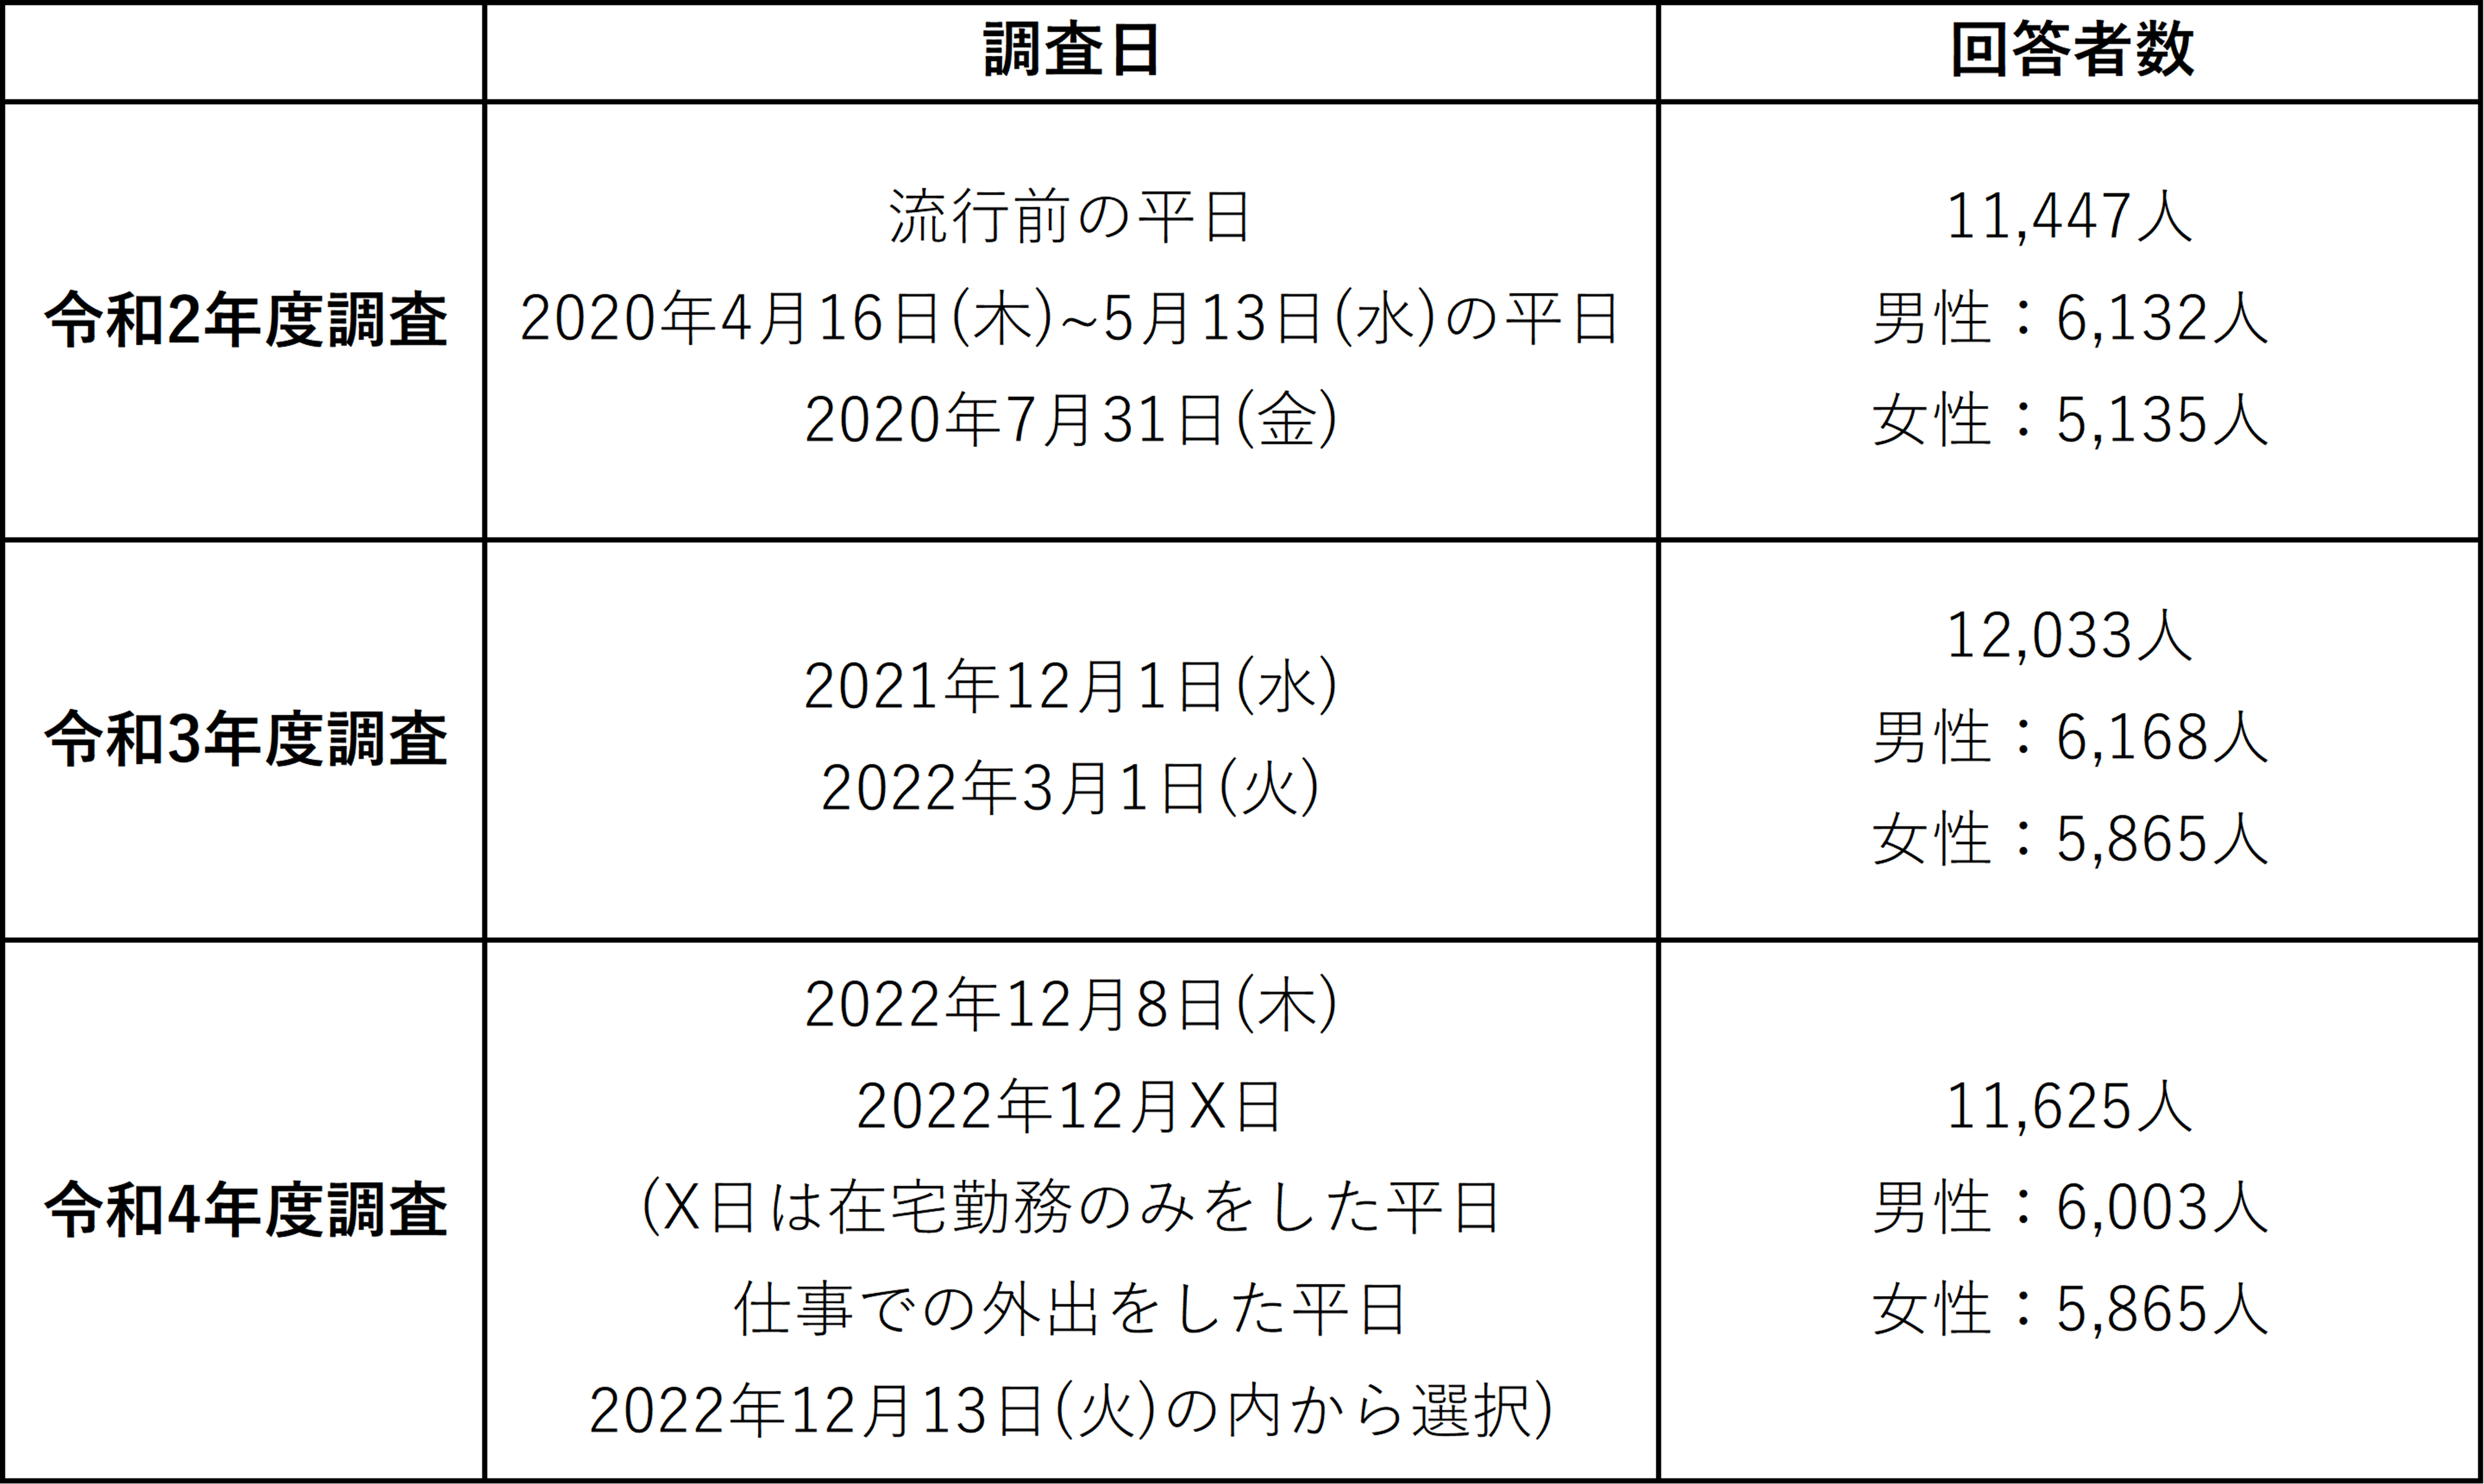
\includegraphics[width=120mm]{figure/c02s01_table_国交省調査の概要.png}
  \label{国交省調査の概要}
\end{table}

%この部分は、「1文1文は短く要点を抑えているが、前後のつながりが分かりくい。」と指摘されたので、要推敲する。
この調査は、令和2年度から4年度にかけて毎年度実施され、調査日は流行前から2022年12月までの7つの時点で行われた。
故に、コロナ禍での時系列的な分析に非常に有用である。
ただし全ての調査日は平日であったため、休日中の行動については考慮できていない。
調査日と社会状況の関連性については第3章で詳しく述べる。\\
 回答者数については概ね11,000人から12,000人の間を推移している。
この調査では前回調査のIDを回答する項目があり、総回答者数は減るが,全ての調査に回答した人(以下,全回答者)を抽出することが可能となる。
そのため、本研究では全回答者のデータを使用する。具体的な対象者の選定については後述する。
また,生活時間調査とアンケート調査は別々の回答者であることに留意したい。
表\ref{国交省調査の概要}の回答者数は生活時間調査の回答者数である。
図\ref{国交省調査の調査地域}は、国交省調査の調査地域を示している。\\

\begin{figure}[H]
  \centering
  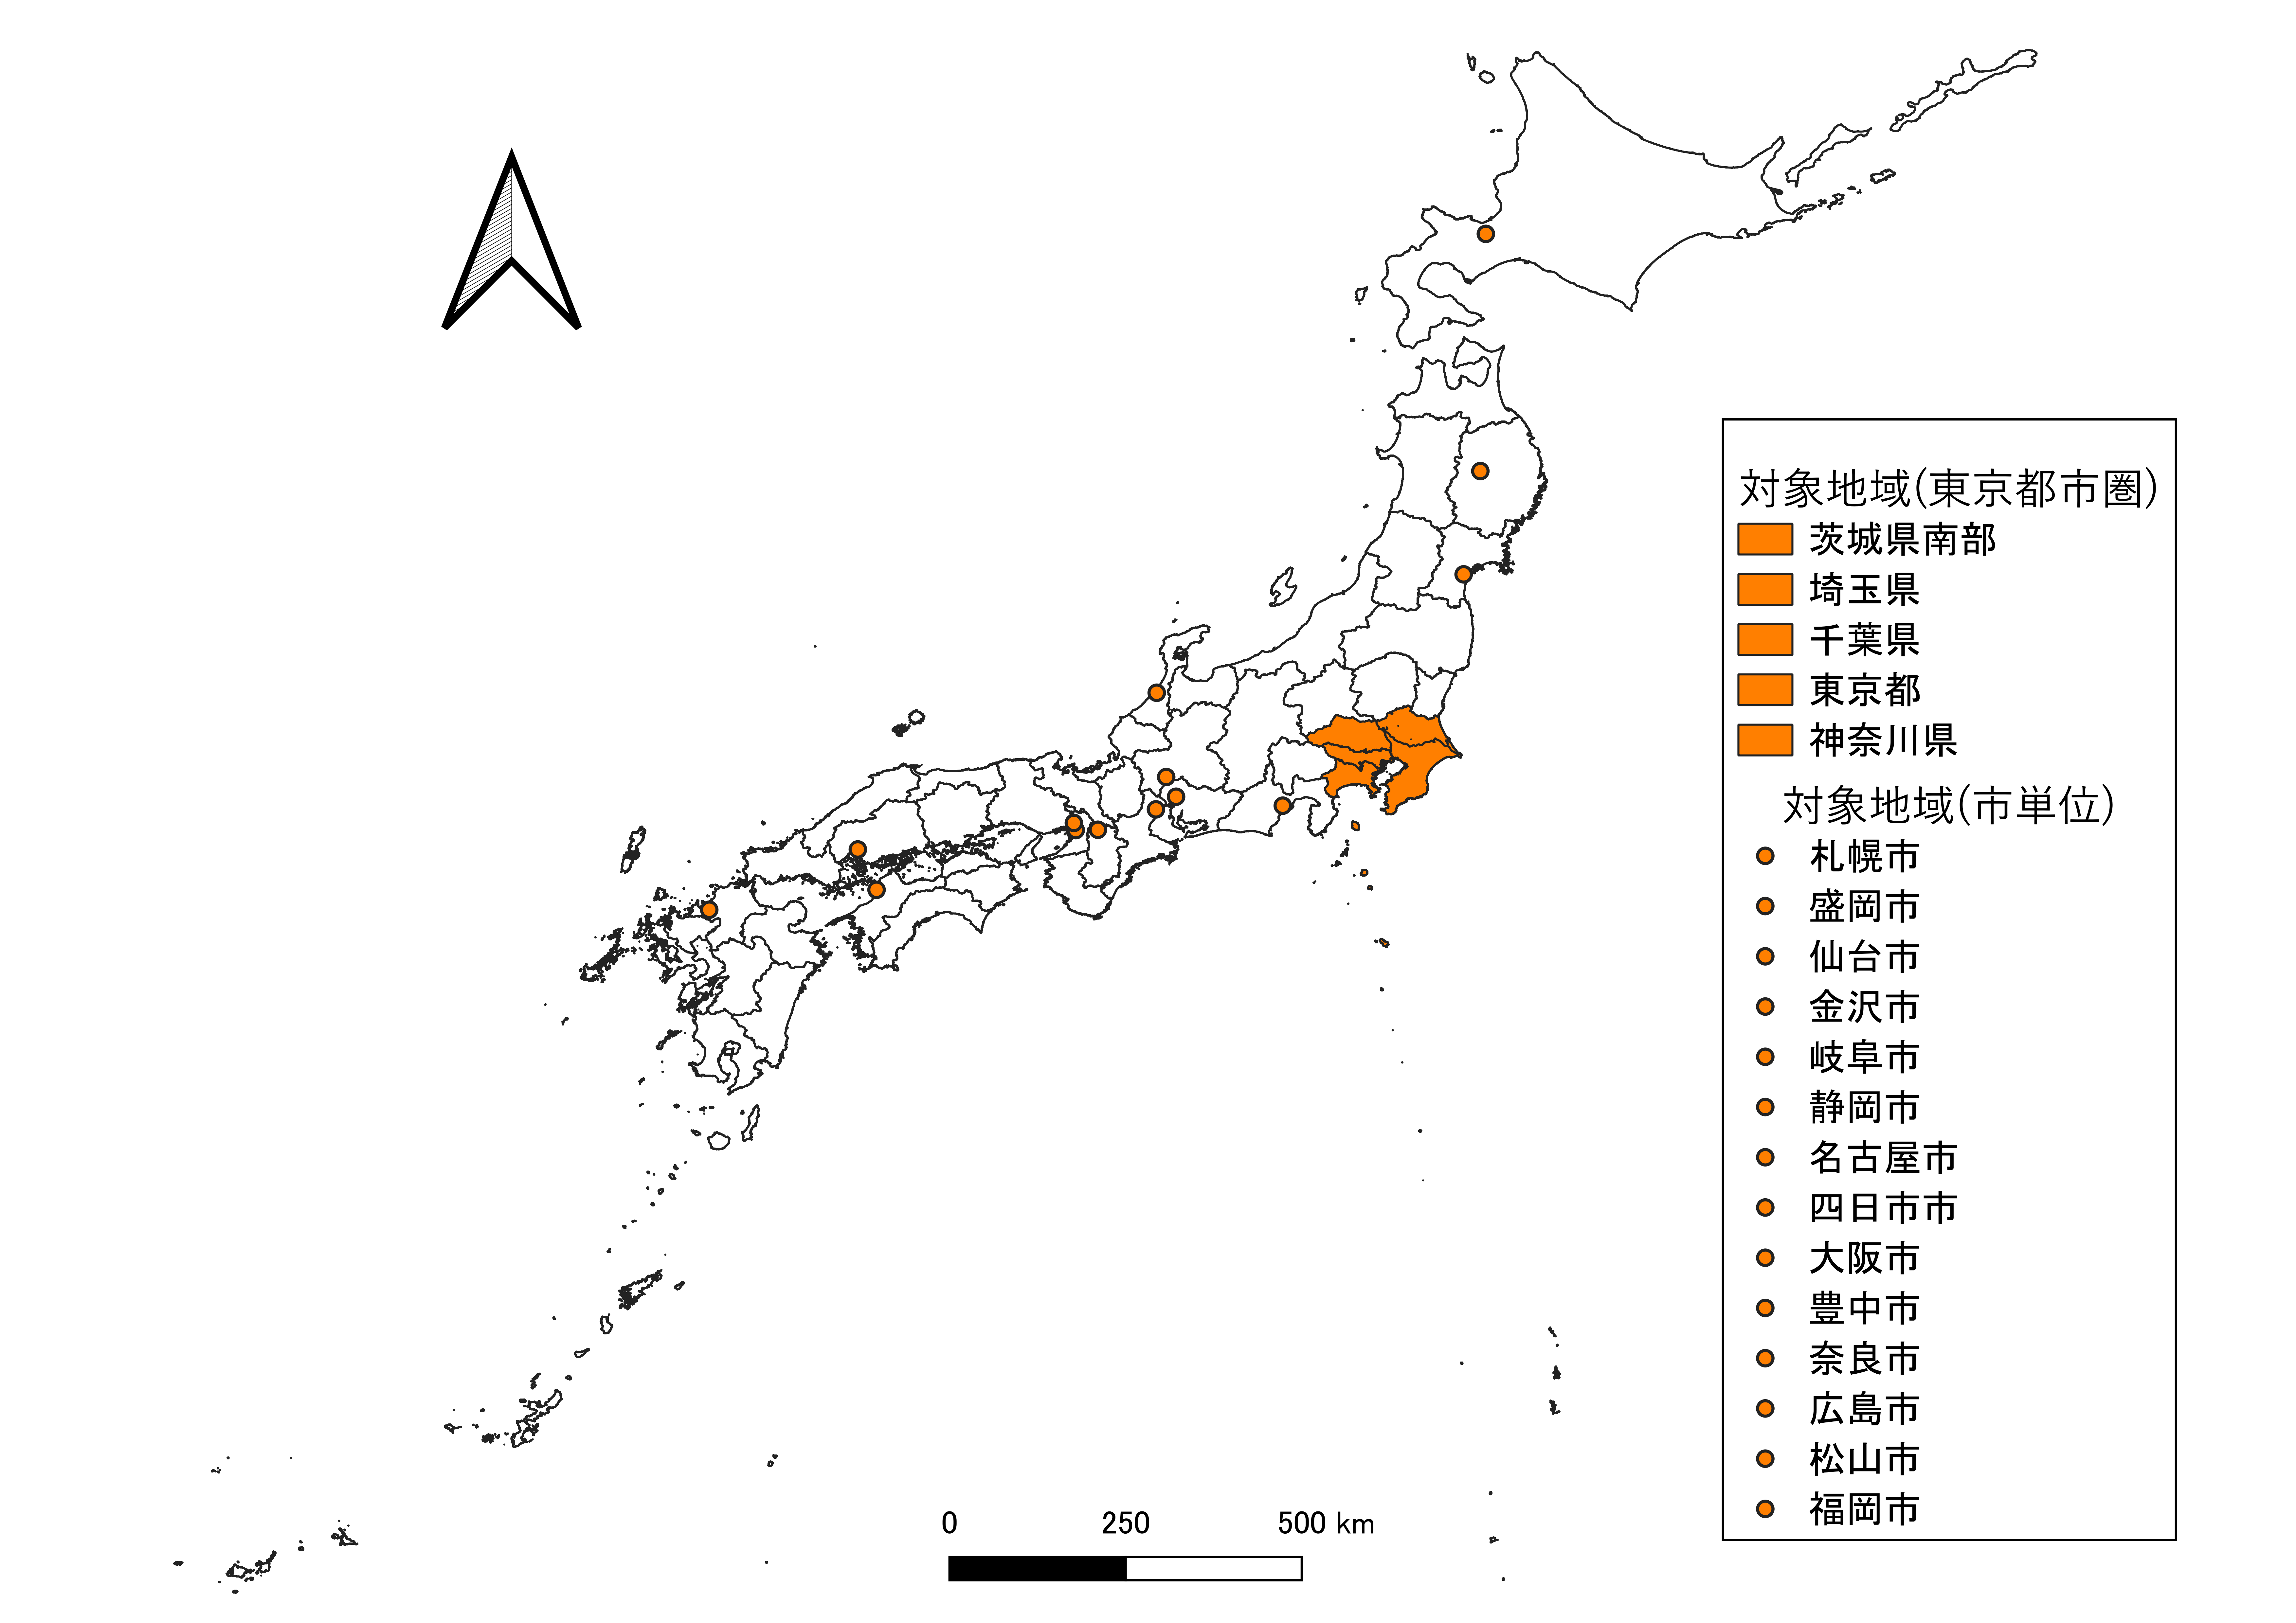
\includegraphics[width=120mm]{figure/c02s01_fig_MLIT-Target-Area-ver3.png}
  \caption{国交省調査における調査地域}
  \label{国交省調査の調査地域}
\end{figure}

調査地域の選定に関して、国交省(2020)は「新型コロナウイルスの感染者が多い東京都市圏及び、全国的な傾向を把握するため、全国都市交通特性調査の対象地域から都市類型や特定警戒都道府県の有無の観点から対象都市を抽出」している。
東京都市圏では茨城県南部以外の地域が県単位で行われている。
その他の対象地域は市単位での調査である。\\
 国交省(2020)によると、令和2年度時点では緊急事態宣言解除後(2020年7月31日)においても自宅で長く過ごす傾向があることや、オンラインやリモート活動の意向は商品購入等が高く、飲み会などのコミュニケーションに関するものは低いという速報結果がある。
これらの結果は全体傾向であるため、社会属性ごとの差異などが不鮮明である。
また、活動時間が増えたことを把握できても、それがどのタイミングで変化しているのかまで分析されていない。
そのような変化は時空間経路図を用いることで表すことが出来る。\\
 国交省調査を用いた研究は少ないものの、岡田(2021)では、テレワークの導入が社会属性によって異なることや、地域内の感染者数の高さと正の相関があることを明らかにしている。
また、石橋(2023)は、PT調査と組み合わせ、働き方や自動車保有状況によってコロナ禍での身体的活動量が異なることを明らかにしている。
これらの研究は令和2年度調査を使用していることが多く、それ以降の調査を用いた研究や、各調査年度を組み合わせて時系列的に分析を行っている研究は少ない。\\
 次に国交省調査に類似するデータとして,総務省統計局が出す社会生活基本調査が挙げられる。
調査形式は、国交省調査と同様にアンケート調査と15分単位の生活時間調査である。
この調査は都道府県単位で行われており、調査頻度は5年毎である。
最新の調査は2021年であり、この調査のみでコロナによる時系列的な影響を捉えるのは難しい。
故に、時系列的な影響を捉えるには国交省調査を使用するのが望ましいだろう。\\
 最後に対象地域と対象者の選定を行う。
前述したように全回答者のデータを使用する。
全回答者の人数は1,550人(男性:955人/女性:595人,1年度あたり)である。
全回答者にすることで,データの整合性が向上し,個々の変化をより正確に捉えることができる。
対象地域は回答者数を確保しつつ,複数地域を比較したいため,回答者数のバラつきが少ない地域を選定する。
コロナ禍で変化を受けた職業従事者や非有職者などを考慮に入れながら,回答者数が多いものを選定する。
図\ref{3年度分の合計人数に基づいた地域分布}は3年度分の回答者を集計し,その合計人数に基づいて地域別に表したものである。\\

\begin{figure}[H]
  \centering
  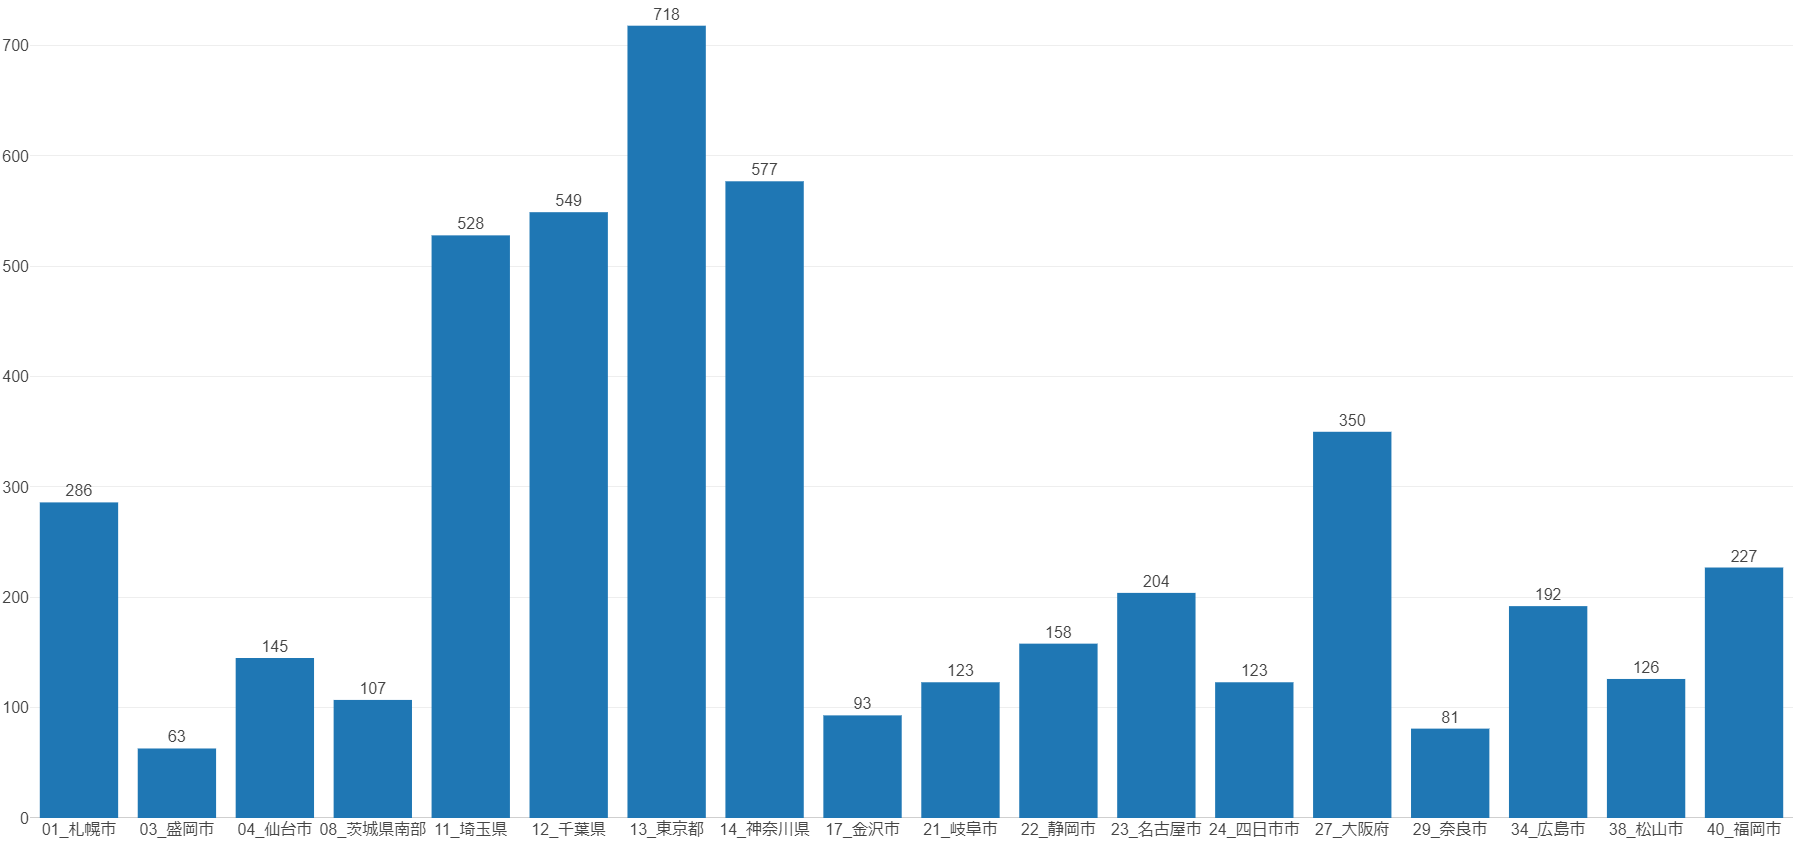
\includegraphics[width=120mm]{figure/c02s01_fig_3年度分の合計人数に基づいた地域分布.png}
  \caption{3年度分の合計人数に基づいた地域分布(単位:人)} %(国交省調査を基に作成)を入れる
  \label{3年度分の合計人数に基づいた地域分布}
\end{figure}

埼玉県,千葉県,神奈川県の3県は550人前後と回答者数も多く,ばらつきも少なく分布しているため,本研究ではこの3県を対象地域とする。
この3県は1都3県の連携を掲げ,足並みを揃えながら感染症対策に取り組んでいた。
そのため,各地域における生活の変容が一様ならば感染症対策によるものとして把握でき,異なれば地域固有のものとして把握できる。
東京都を除いた理由としては,回答者数が極めて多い上,3県と比べ経済規模や人口規模が明らかに異なるからだ。
表\ref{対象地域の調査年度毎の回答者数}は対象地域の回答者数を表したものである。\\

\begin{table}[H]
  \centering
  \caption{対象地域の調査年度毎の回答者数(単位:人)} %(国交省調査を基に作成)を入れる
  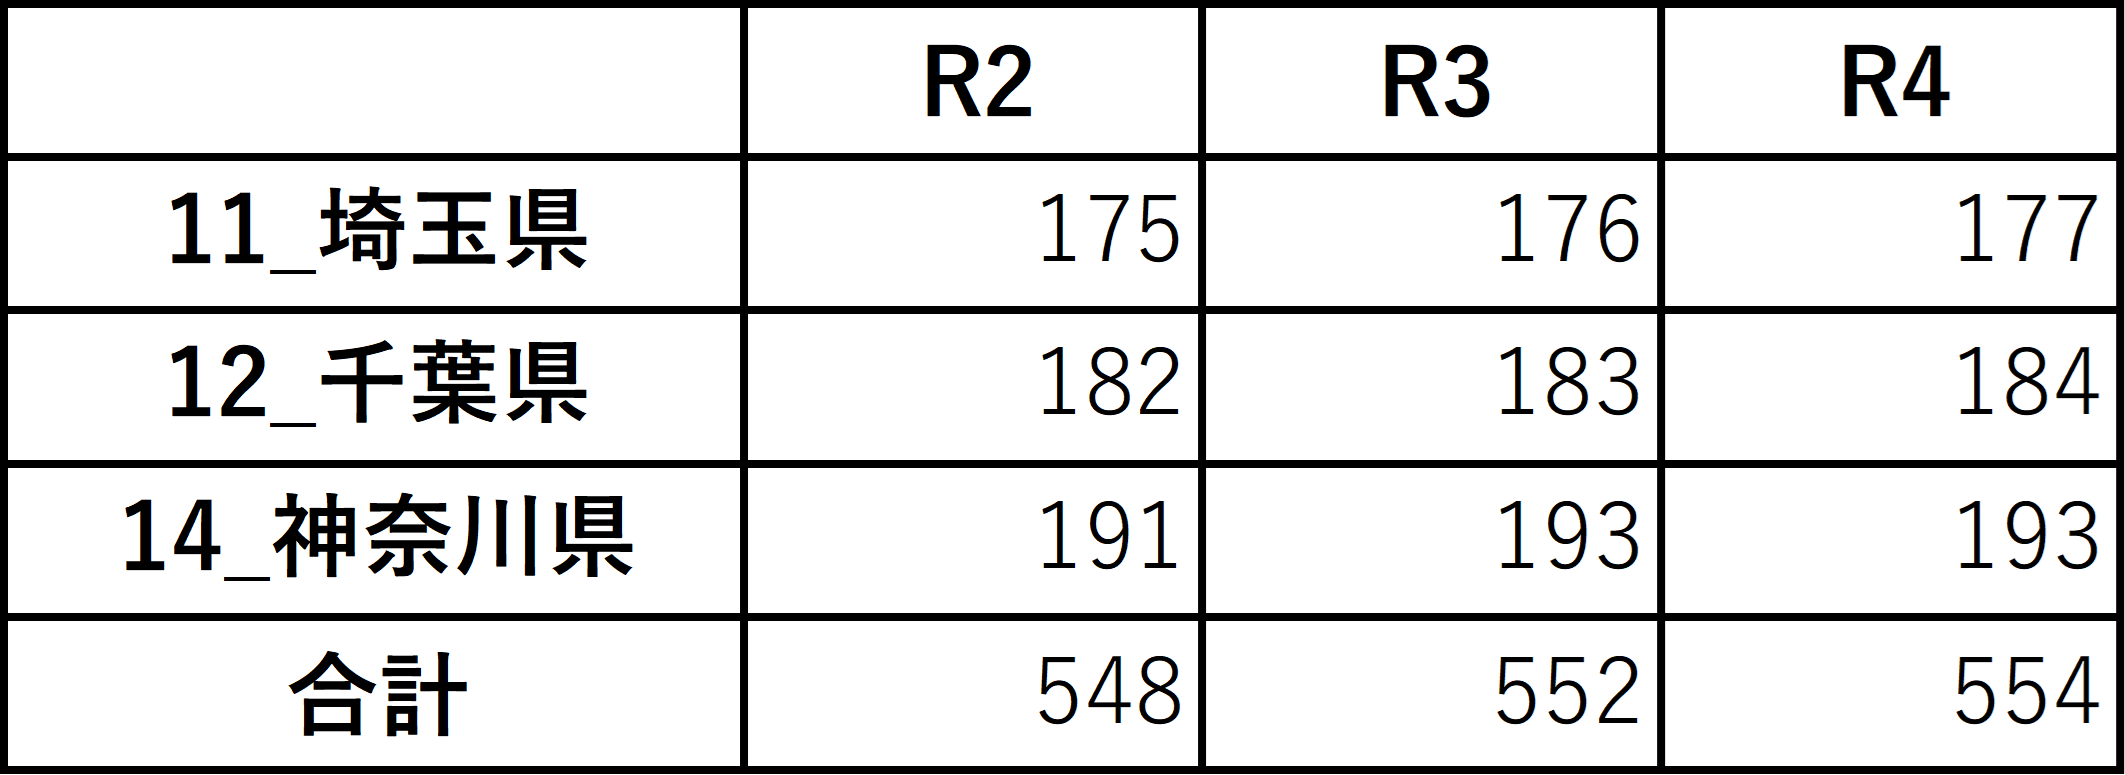
\includegraphics[width=90mm]{figure/c02s01_table_対象地域の調査年度ごとの回答者数.png}
  \label{対象地域の調査年度毎の回答者数}
\end{table}

図\ref{対象地域内における社会属性の人数と男女構成}は令和2年度調査時点における対象地域内での社会属性の数とその男女構成である。
その他の調査年度も同様の傾向を示しているため,令和2年度調査のみで選定をした。
各職業の定義は総務省の定める日本標準職業分類に基づいている。
最も多い回答者は無職であり,次いで主婦・主夫(以下,主婦)と非有職者が多いことが分かる。\\
 しかし,職業従事者に関しても時空間の変容が起きている可能性があるため,分析を行うべきである。
したがって,次点で回答者の多い事務従事者や管理的職業従事者,専門的・技術的職業従事者も対象者として含める。
加えて,対面接触を必要とする職業従事者としてサービス職業従事者も含める。\\

\begin{figure}[H]
  \centering
  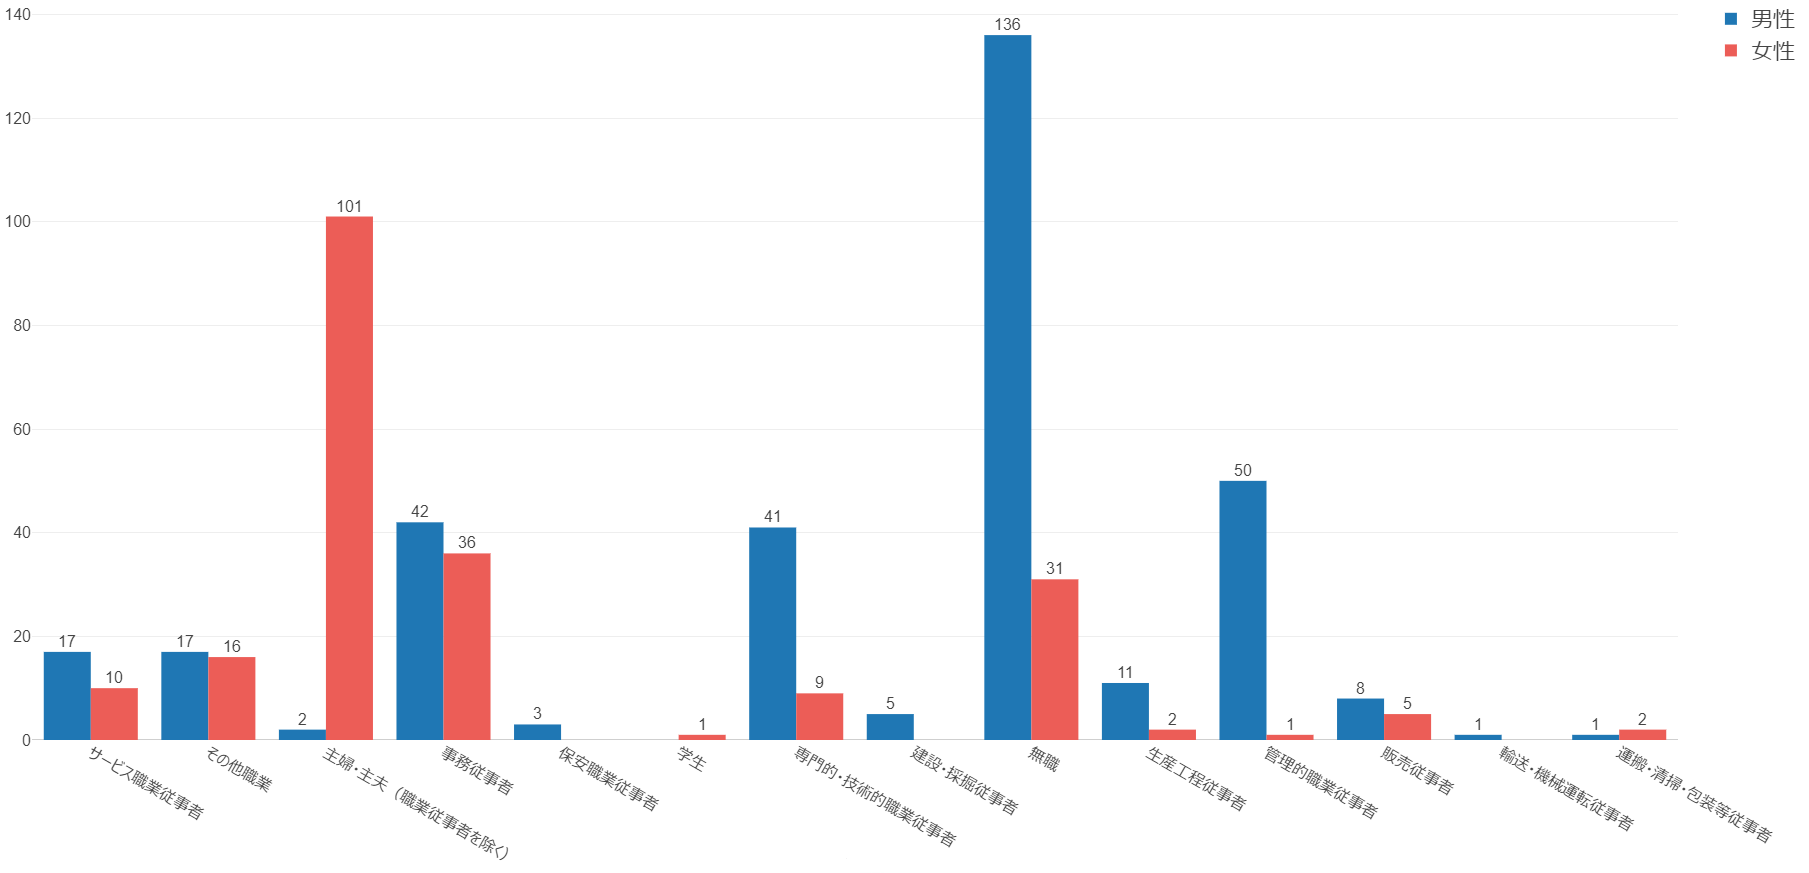
\includegraphics[width=120mm]{figure/c02s01_fig_対象地域内における社会属性の人数とその男女構成_2020.png}
  \caption{対象地域における社会属性の人数と男女構成(単位:人)} %(国交省調査を基に作成)を入れる
  \label{対象地域内における社会属性の人数と男女構成}
\end{figure}

また,主婦に関しては,男女数を考慮して女性のみを対象とする。
そして,無職に関しては,図\ref{無職の回答者区分}に示しているように60歳以上の男性が最も多い。
このような特徴に該当する社会属性として挙げられるのは,定年退職者である。
そのため,本研究においては無職から60歳以上の男性のみを抽出し,定年退職者として扱い分析を行う。\\

\begin{figure}[H]
  \centering
  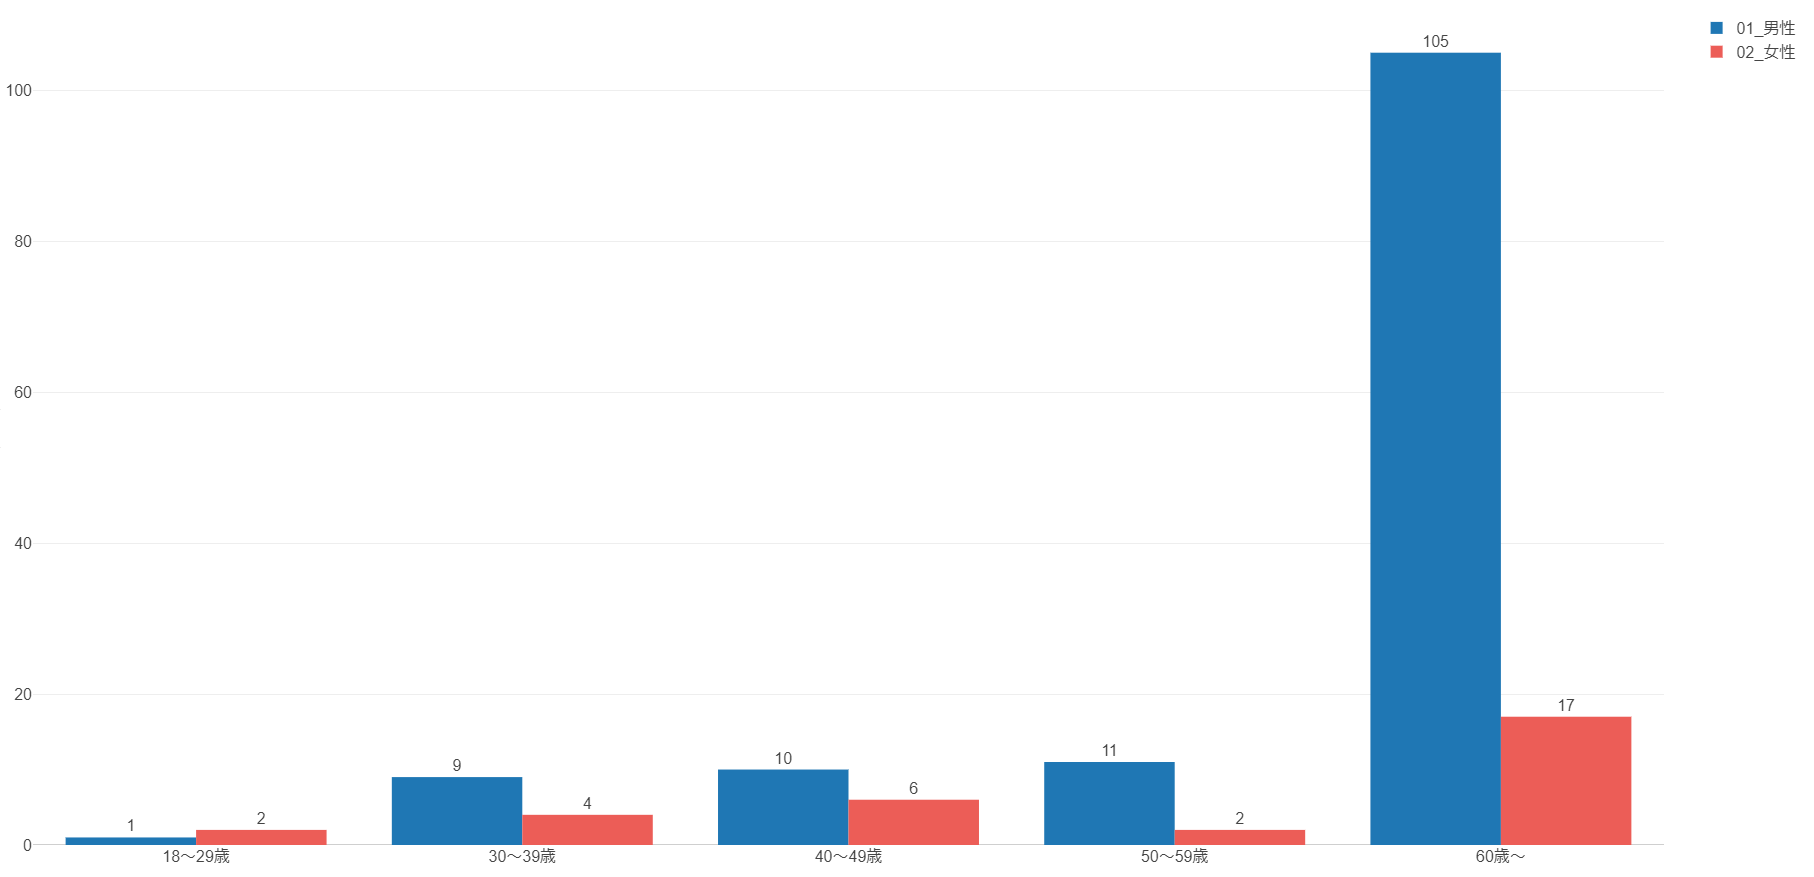
\includegraphics[width=120mm]{figure/c02s01_fig_定年退職者の選定.png}
  \caption{男女別・年齢別の無職の回答者数(令和2年度調査)(単位:人)} %(国交省調査を基に作成)を入れる
  \label{無職の回答者区分}
\end{figure}

したがって,本研究での対象地域は埼玉県,千葉県,神奈川県の3県であり,対象者は事務従事者,管理的職業従事者,専門的・技術的職業従事者,サービス職業従事者,主婦,定年退職者の計6つの社会属性の人々とする。\\

\subsection{新型コロナウイルスの影響下における生活意識・行動の変化に関する調査}

内閣府調査は,内閣府がコロナ禍において人々の生活意識や行動がどのように変化したのかを把握する目的で行った調査である。
調査形式はWeb上でのアンケート調査である。
表\ref{内閣府調査の概要}は本研究で使用する調査日,回答者数,調査地域を表したものである。
実施された回数は,2020年6月21日,2020年12月24日,2021年6月4日,2021年11月1日,2022年7月22日,2023年4月19日の計6回である。
本研究では,2020年6月21日から2021年11月1日の計4回の調査を使用する。\\

\begin{table}[H]
  \caption{内閣府調査の概要}
  \centering
  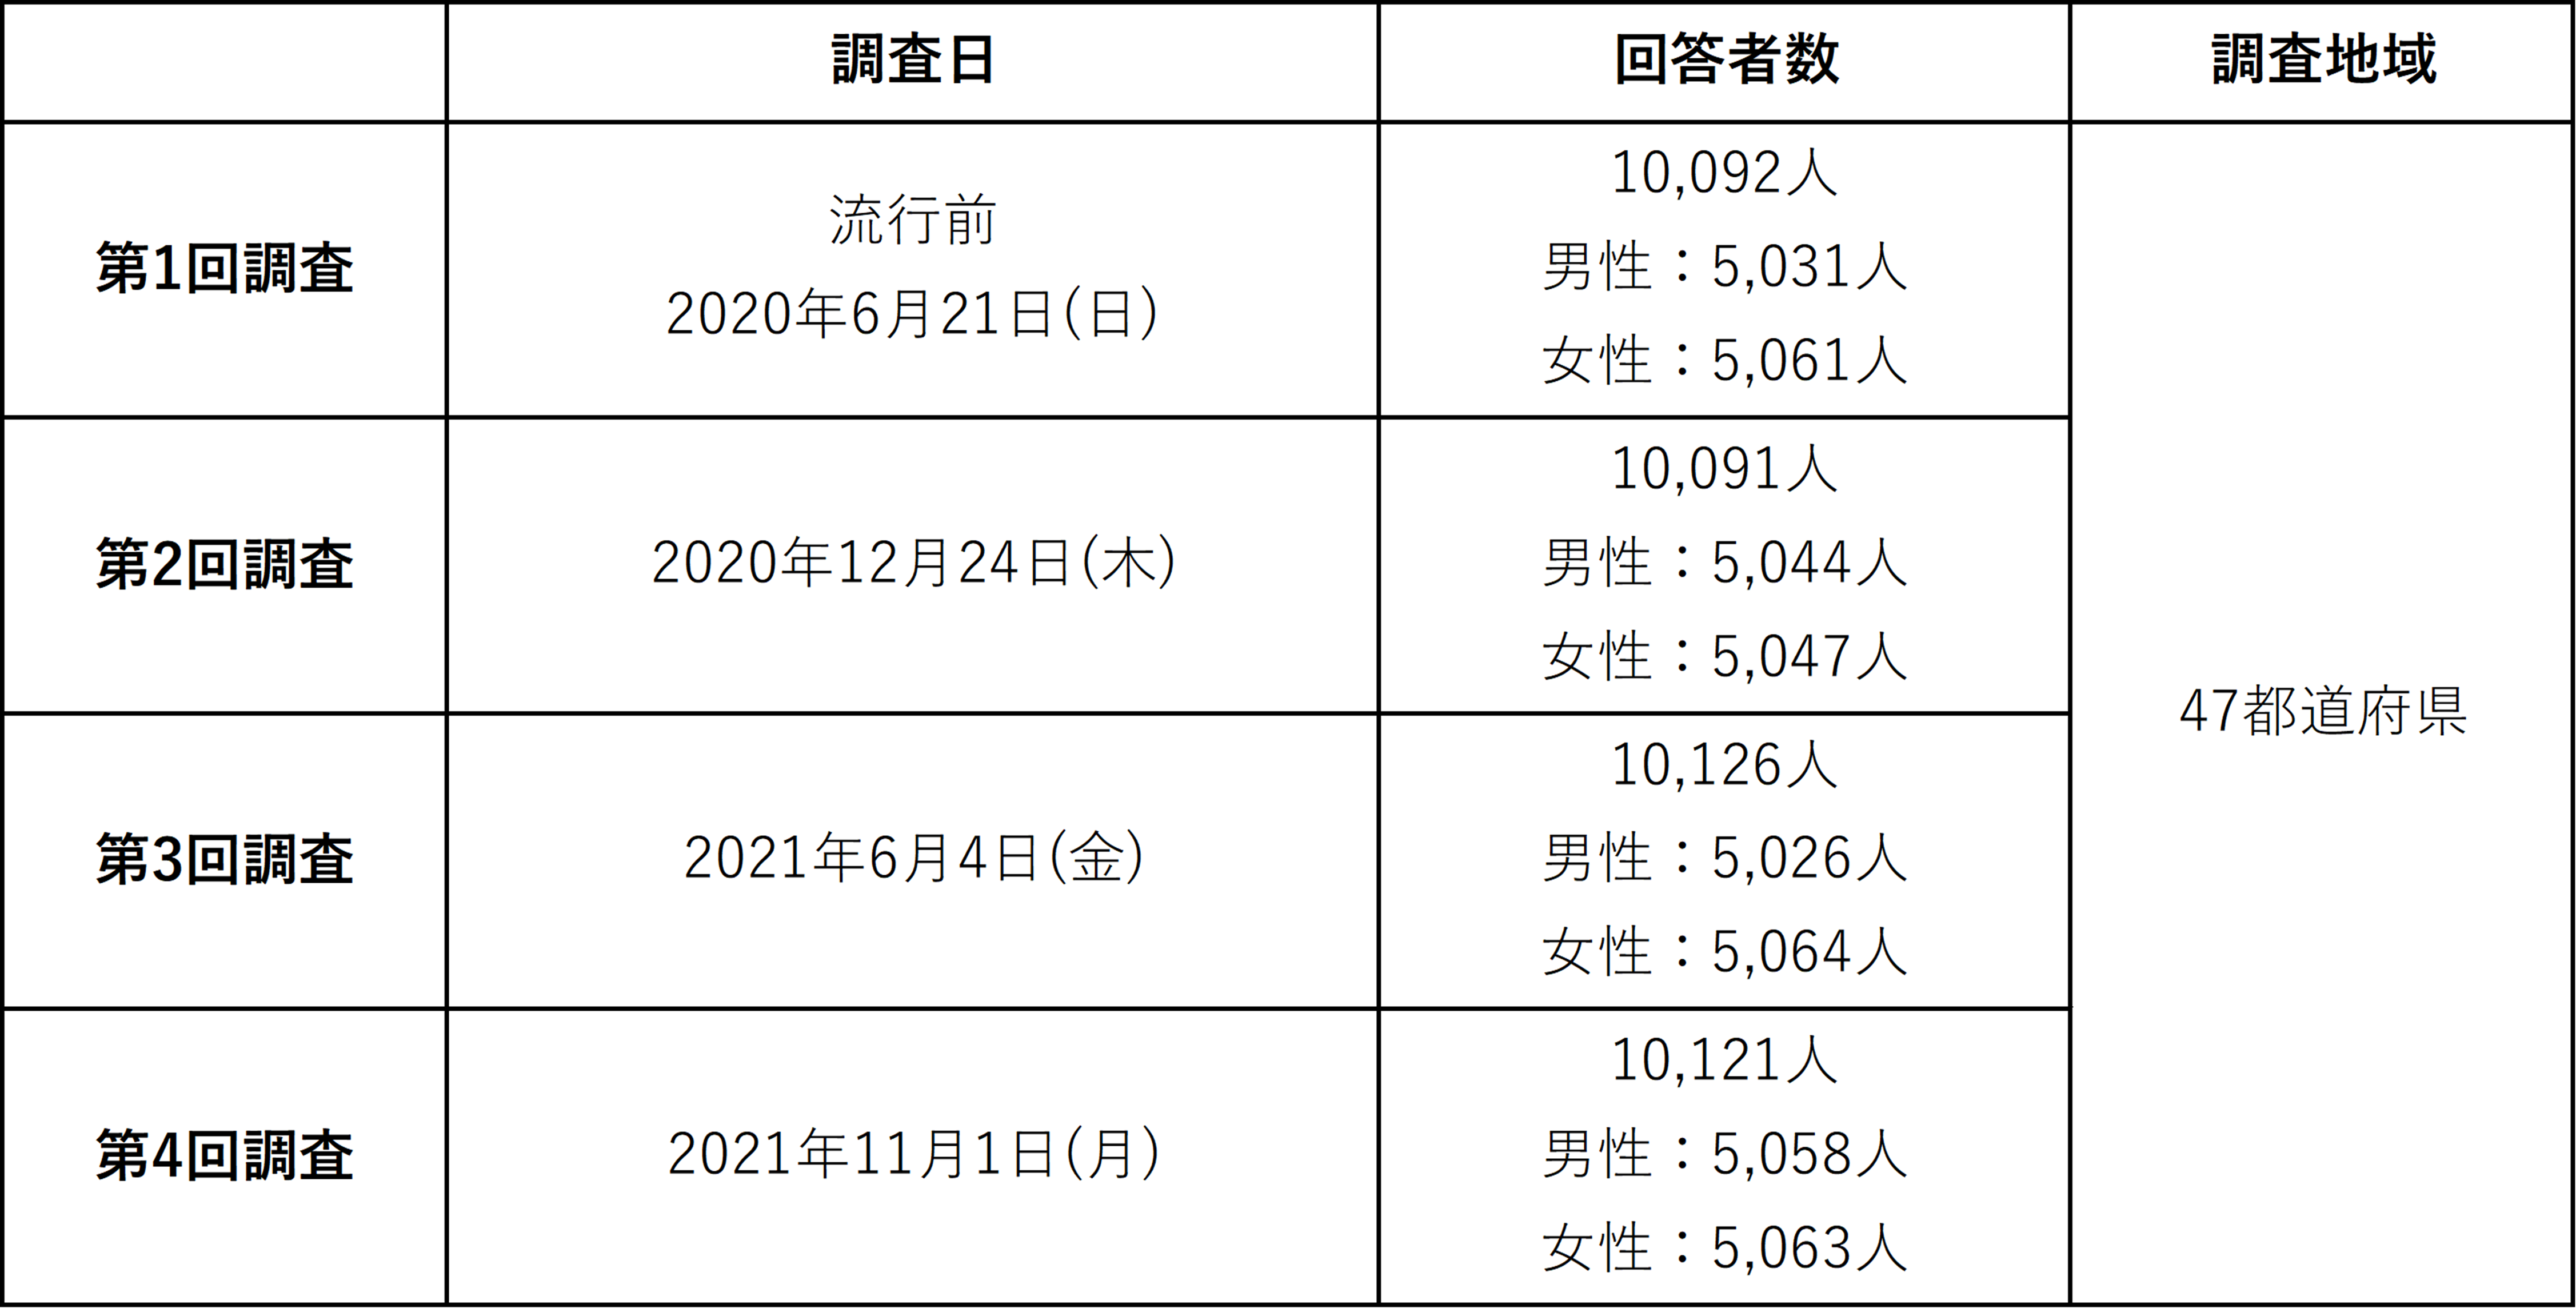
\includegraphics[width=120mm]{figure/c02s02_table_内閣府調査の概要.png}
  \label{内閣府調査の概要}
\end{table}

回答者数は約10,000人が回答している。
国交省調査と同様にIDの追跡が可能であり,全回答者を抽出することが出来る。
本研究では,内閣府調査も全回答者のデータを使用する。
調査地域は都道府県単位で行われている。
対象地域や対象者は国交省調査を基準とする。
留意点として,内閣府調査は業種別で職業が分類されているが,職業分類自体は総務省の定める日本標準職業分類に基づいているため整合性を取ることは可能である。
調査日については,第3章で社会状況と関連させながら述べる。\\
 この調査を使用する目的としては,時間地理学的に分析をする国交省調査を補強するためである。
時間地理学の弱点として,人の内面についての理解が出来ない点がある。
時空間経路図を利用して時空間的な不利益や不平等を把握できるものの,そのような状況下で人々がどのような思いを持っているのかを把握できない。
それ故,時間地理学の研究ではアンケート調査と組み合わせることが多い。
本研究でも同様に,内閣府調査を用いて内面的な部分を補うこととする。\\
 前述したように国交省調査でもアンケート調査が行われているが,回答者が異なる。
さらに,質問内容は活動頻度や外出する場所などの生活時間調査を設問形式に直したようなものが多い。
内閣府調査も国交省調査における生活時間調査の回答者と異なっている。
しかし,国交省調査のアンケート調査に比べ,生活の満足度や,テレワークに関する意識,家事・育児の役割変化,移住への関心などの生活意識に関わる質問内容が多い。
そのため,内閣府調査は国交省調査のアンケート調査よりも内的な側面を補うものとして有用である。\\

\section{コロナによる社会状況の変化}

この章では,始めに代表的な感染症対策の特徴を述べ,その後2020年から2022年までのコロナによって変化した社会状況について整理する。\\

\subsection{代表的な感染症対策について}

代表的な感染症対策として挙げられるものは,緊急事態宣言,まん延防止等重点措置,BA5対策強化宣言の3つである。
図\ref{代表的な感染症対策の特徴}では,各対策の特徴について内閣感染症危機管理統括庁や自治体の資料等を基に整理して示した。\\

\begin{figure}[H]
  \centering
  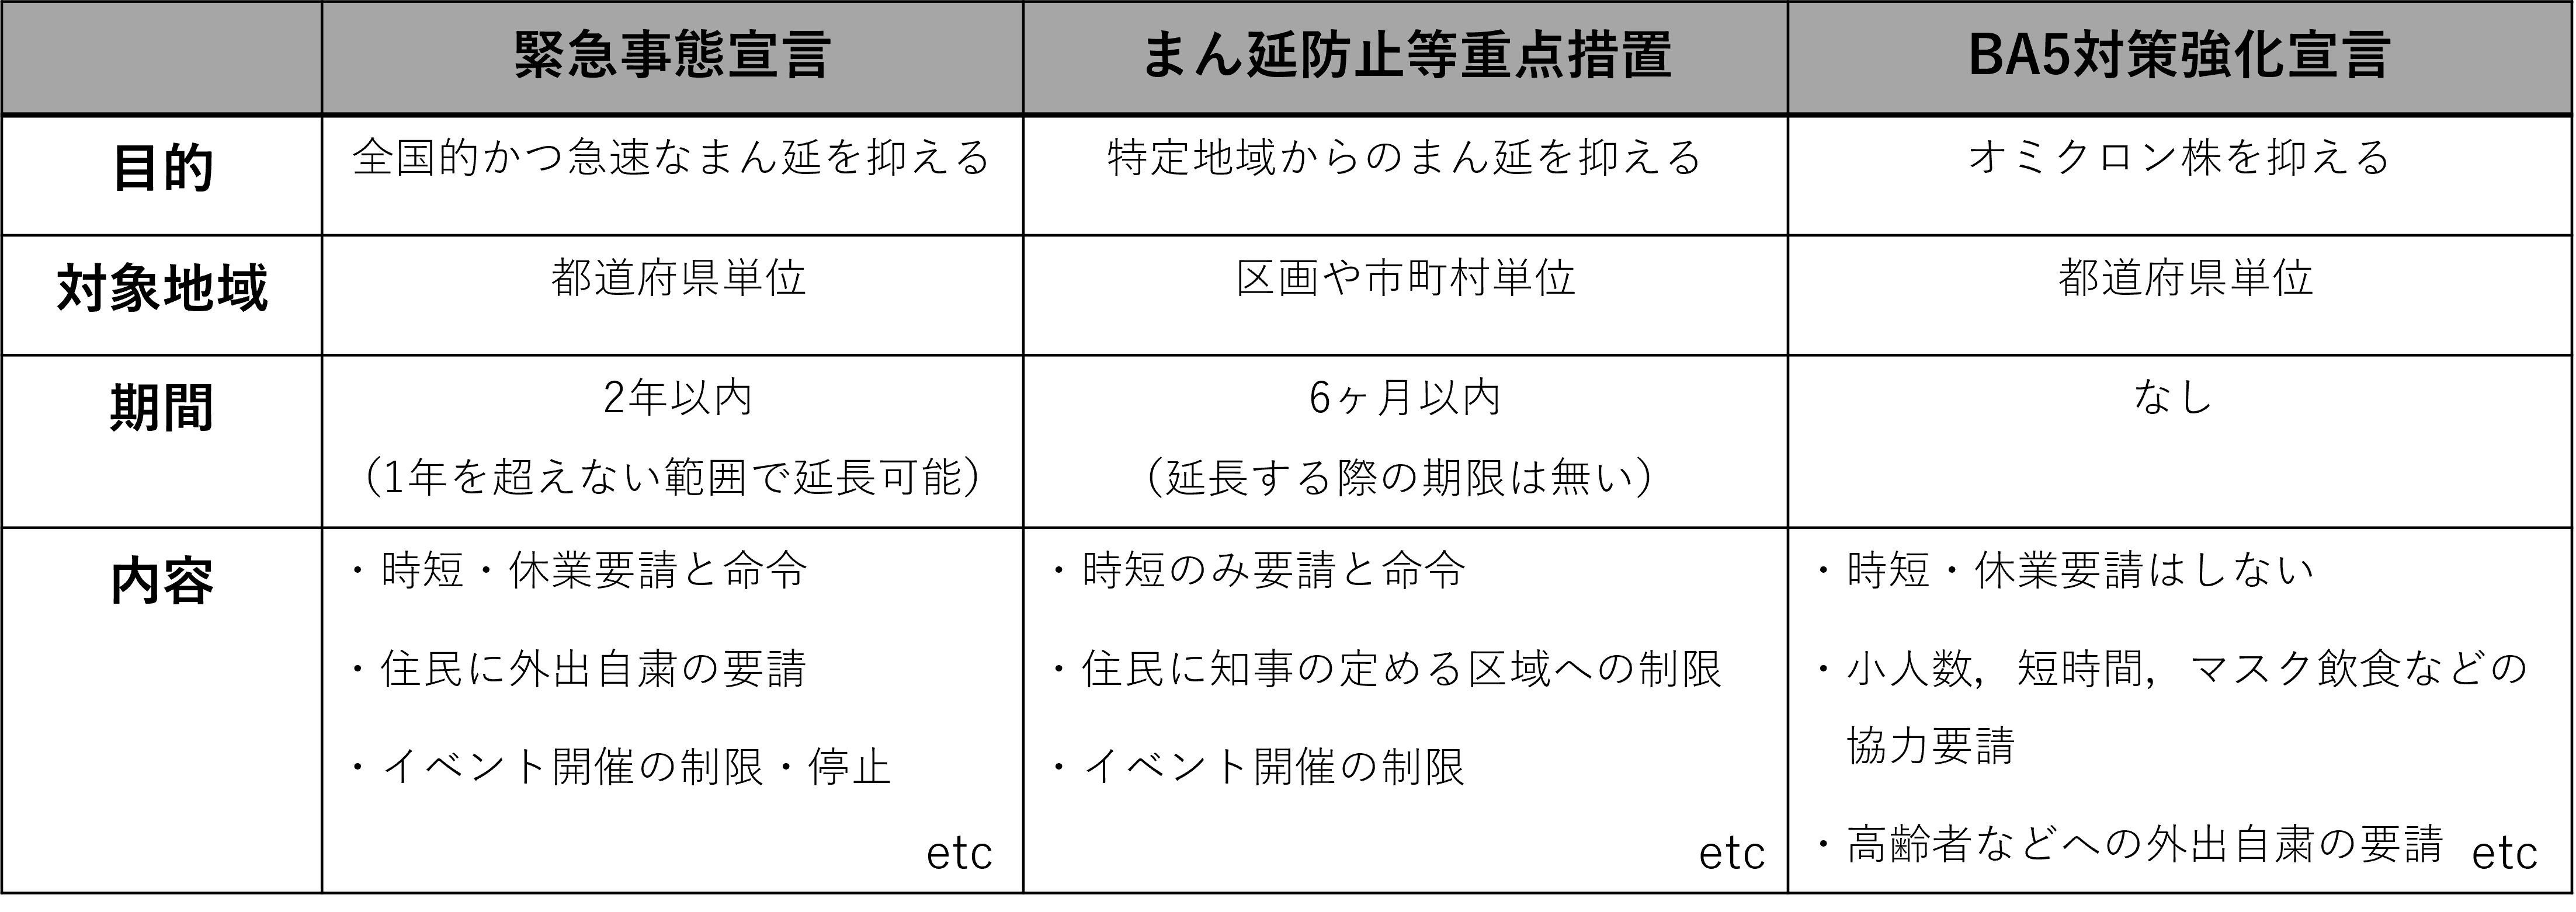
\includegraphics[width=120mm]{figure/c03s01_fig_各感染症対策の違い.png}
  \caption{代表的な感染症対策の特徴}
  \label{代表的な感染症対策の特徴}
\end{figure}

緊急事態宣言は,都道府県単位で時短・休業要請を指示することが出来る。
他の対策と異なる点として,休業要請やイベントの停止が取れる点と外出自体に自粛要請を取れる点がある。
前者は営業自体を止められるため,サービス職業従事者のような職業は時空間的に大きな制約を受ける可能性がある。
後者は「自粛」という諸外国に比べ強制力が低いものではあるが,廣井(2020)の研究では,様々な社会属性の人々,特に主婦や高齢者は外出を控えるようにしていた。
そのため,外出自粛の影響は大きいといえる。\\
 まん延防止等重点措置は,緊急事態宣言より制限が弱い。
緊急事態宣言による制限は社会経済的活動に大きな支障をもたらすため,ある程度活動を維持しながら感染症対策を行っていくことが狙いにある。
期間は6ヶ月以内と短いものの,延長期間の際限が無いことで時間の調整がしやすい。
それ故,まん延防止等重点措置は柔軟な対応を取れるという利点がある。\\
 BA5対策強化宣言は,他2つの対策とは目的が異なり,オミクロン株の流行を抑えるための限定的な対策である。
対象地域は都道府県単位と広範でありながらも,その強制力は極めて低い。
これは,感染力は強いが,重症化しにくい特徴をもつBA5というオミクロン株の一種が当時流行していたことと関係がある。
感染リスクの高い行動を控えるよう促すのみにし,時短・休業要請のような社会経済的活動に支障が出る制限は行わない方針で作られた感染症対策である。
しかしながら,免疫力があまりない高齢者や基礎疾患を持つ人々は重症化しやすいので外出自粛の要請を行う形が取られている。\\
 図\ref{感染症対策における適用地域}では,上記3つの感染症対策における適用地域の分布を表したものである。
第1回緊急事態宣言の凡例における最初期とは2020年4月7日時点である。
最後期は2020年4月16日の適用地域を拡大した時点のものである。
まん延防止等重点措置における適用とは,端を発した2021年4月頃から各種対策が一斉に解除される同年の9月末までにまん延防止等重点措置を実施した地域である。
BA5対策強化宣言における適用とは,端を発した2022年7月末から同年8月までにBA5対策強化宣言を実施した地域である。\\

\begin{figure}[H] %この図の位置は要調整
  \centering
  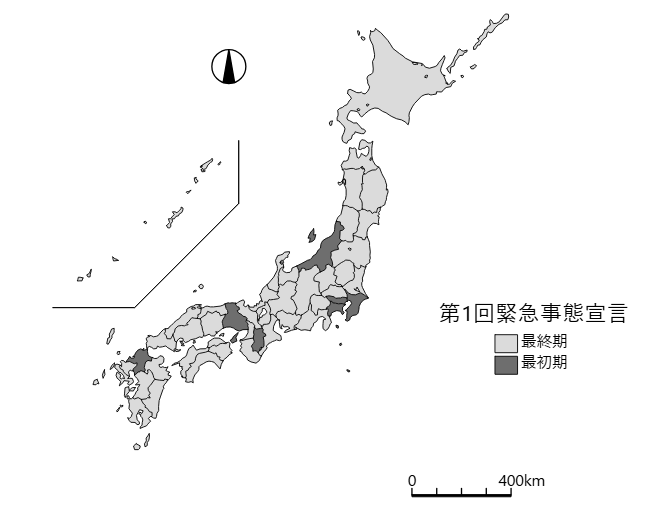
\includegraphics[width=85mm]{figure/c03s01_fig_感染症対策適用地域_01.png}
  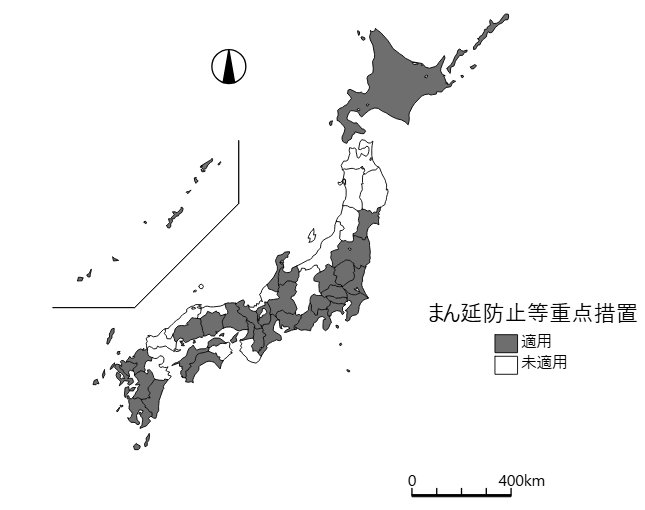
\includegraphics[width=85mm]{figure/c03s01_fig_感染症対策適用地域_02.png}
  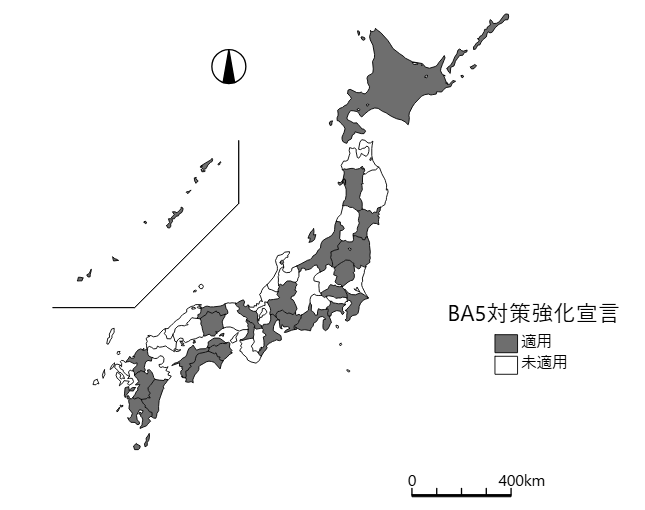
\includegraphics[width=85mm]{figure/c03s01_fig_感染症対策適用地域_03.png}
  \caption{感染症対策における適用地域}
  \label{感染症対策における適用地域}
\end{figure}

第1回緊急事態宣言は最終的に47都道府県の全てに適用されている。
まん延防止等重点措置において,東北地方や中部地方の一部では実施されていないことが分かる。
BA5対策強化宣言では,まん延防止等重点措置より実施された地域は減っているものの,離散的に実施されていることが分かる。\\

\subsection{コロナ禍における感染症対策や主な出来事}

次に,コロナ禍の時系列的な流れを概観する。
表\ref{コロナに関する出来事}では,2020年から2022年までにコロナに関する出来事や実施された感染症対策,そして調査データの実施日を示したものである。\\

\begin{table}[H]
  \centering
  \caption{2020年から2022年までのコロナに関する出来事}
  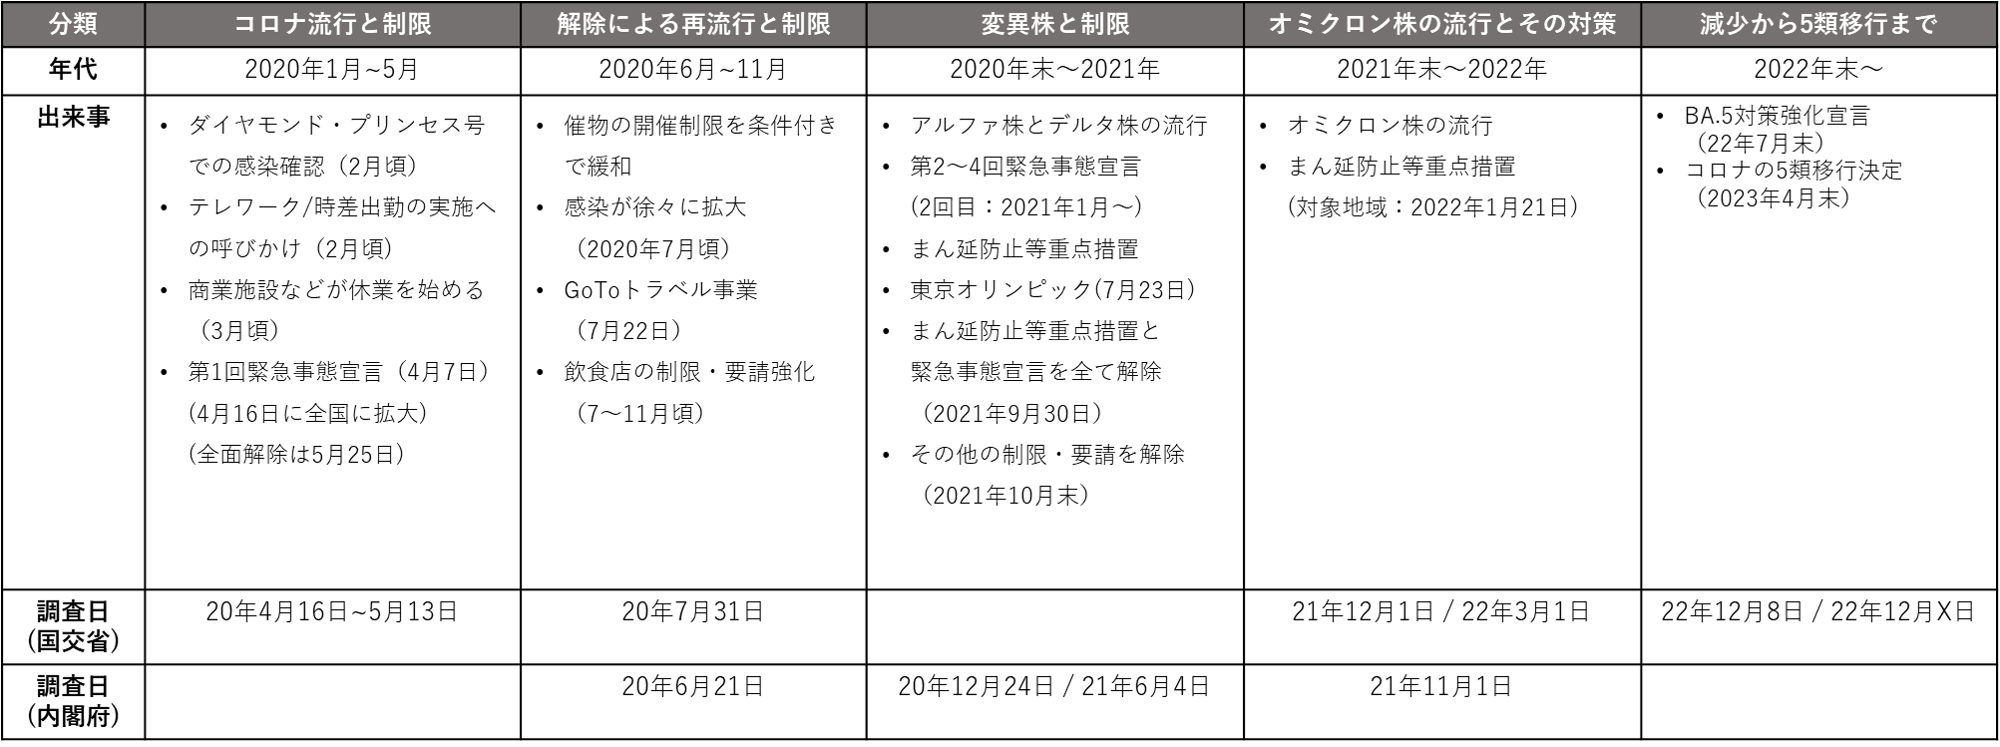
\includegraphics[width=120mm]{figure/c03s02_fig_コロナに関する社会状況の整理.png}
  \label{コロナに関する出来事}
\end{table}

コロナの始まりは2019年末に中国の武漢で発見された原因不明の感染症であった。
日本で周知されるようになった大きなきっかけは,2020年2月頃に起きたクルーズ船「ダイヤモンド・プリンセス号」による感染拡大だろう。
それ以降,徐々に感染症は拡大していき,同年4月から日本で初となる緊急事態宣言が発出された。
しかし,感染症の勢いが収束することはなく,感染拡大と対策が何度も取り組まれた。\\
 2021年からはアルファ株を端とする従来よりも感染力の強い変異株が登場し,より一層感染が拡大していった。
また,同年7月には,延期していた東京オリンピックを開催するなど,ある程度の社会経済的活動を行うようにもなった。
最終的に2023年4月頃にコロナは5類に移行することになった。\\
 国交省調査の調査日を見ると,2回目から4回目までの緊急事態宣言が発出された期間の調査が行われていない。
したがって,緊急事態宣言による時空間的な変容については,コロナ流行前,2020年4月16日~5月13日と2020年7月31日の3時点を対象とする。
まん延防止等重点措置については,2022年3月1日の調査日が発出中に行われた唯一の時点であるため,この時点を対象とする。
そして,BA5対策強化宣言は2022年9月末に解除されているため,解除後の2022年12月頃の2つの調査日を対象とし,解除後の影響を分析する。
特異な時点として,2021年12月1日がある。
この調査日は,2021年9月から10月にかけて緊急事態宣言を含む様々な感染症対策や要請が解除されている時期の直後であるため,コロナ禍でありながら制限を一切受けていない時点として見ることができる。\\
 内閣府調査の方では,2020年6月21日が緊急事態宣言解除の直後の時点である。
2020年12月24日は緊急事態宣言解除後から半年が経った時点である。
2021年6月4日はまん延防止等重点措置下の時点である。
2021年11月1日は2021年10月末の各種制限・要請の全面解除の直後の時点である。
BA5対策強化宣言下の調査日はないことに留意したい。\\

\section{国交省調査の調査分析結果}

この章では,国交省調査を基に行動フラグの選定について述べ,その後各社会属性の分析結果を述べる。
図\ref{行動フラグの選定}は行動フラグの選定過程を示している。
選定を行った理由は、行動フラグごとの平均時間を算出した際に、行動フラグ間でバラつきが大きかったからだ。\\
 活動自体を行っていなかったり,特定の個人のみ行っていたりするものは削除した。
統合したものは,全て家事・育児に関連するものである。
統合前では行動フラグ14や16などと比較する際に,細分化されているため比較が難しくなる。
そのため,今回は行動フラグ17「家事・育児」として一つに統合した。\\
%元々の行動フラグは31種類であり,選定後は17種類となった。

\begin{figure}[H]
  \centering
  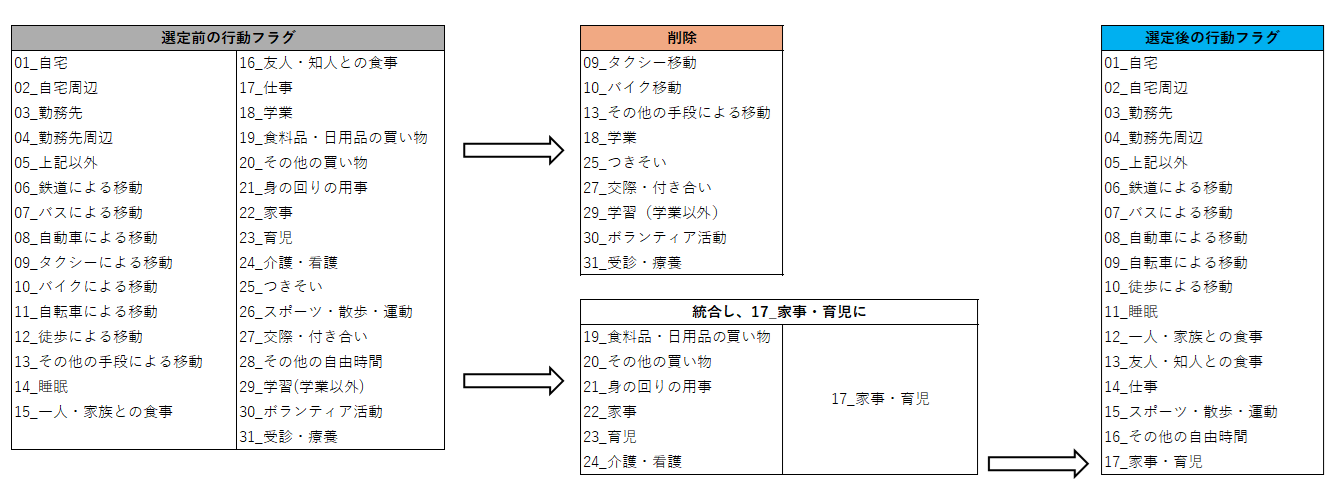
\includegraphics[width=120mm]{figure/c04_fig_行動フラグの選定過程.png}
  \caption{国交省調査における行動フラグの選定過程}
  \label{行動フラグの選定}
\end{figure}

\subsection{事務従事者}

事務従事者は,「一般に課長(課長相当職を含む)以上の職務にあるものの監督を受けて,庶務・文書・人事・調査・企画・会計などの仕事に従事するもの及び生産関連・営業販売・外勤・運輸・通信に関する事務並びに事務用機器の操作の仕事に従事するもの」(総務省,2009,p127)と定義されている。
所謂,サラリーマンなどが該当し,デスクワークが基本となる職業である。
表\ref{sample_事務従事者}は,国交省調査における地域別の事務従事者の就業形態を表した。\\

\begin{table}[H]
  \centering
  \caption{事務従事者のサンプル数(単位:人)}
  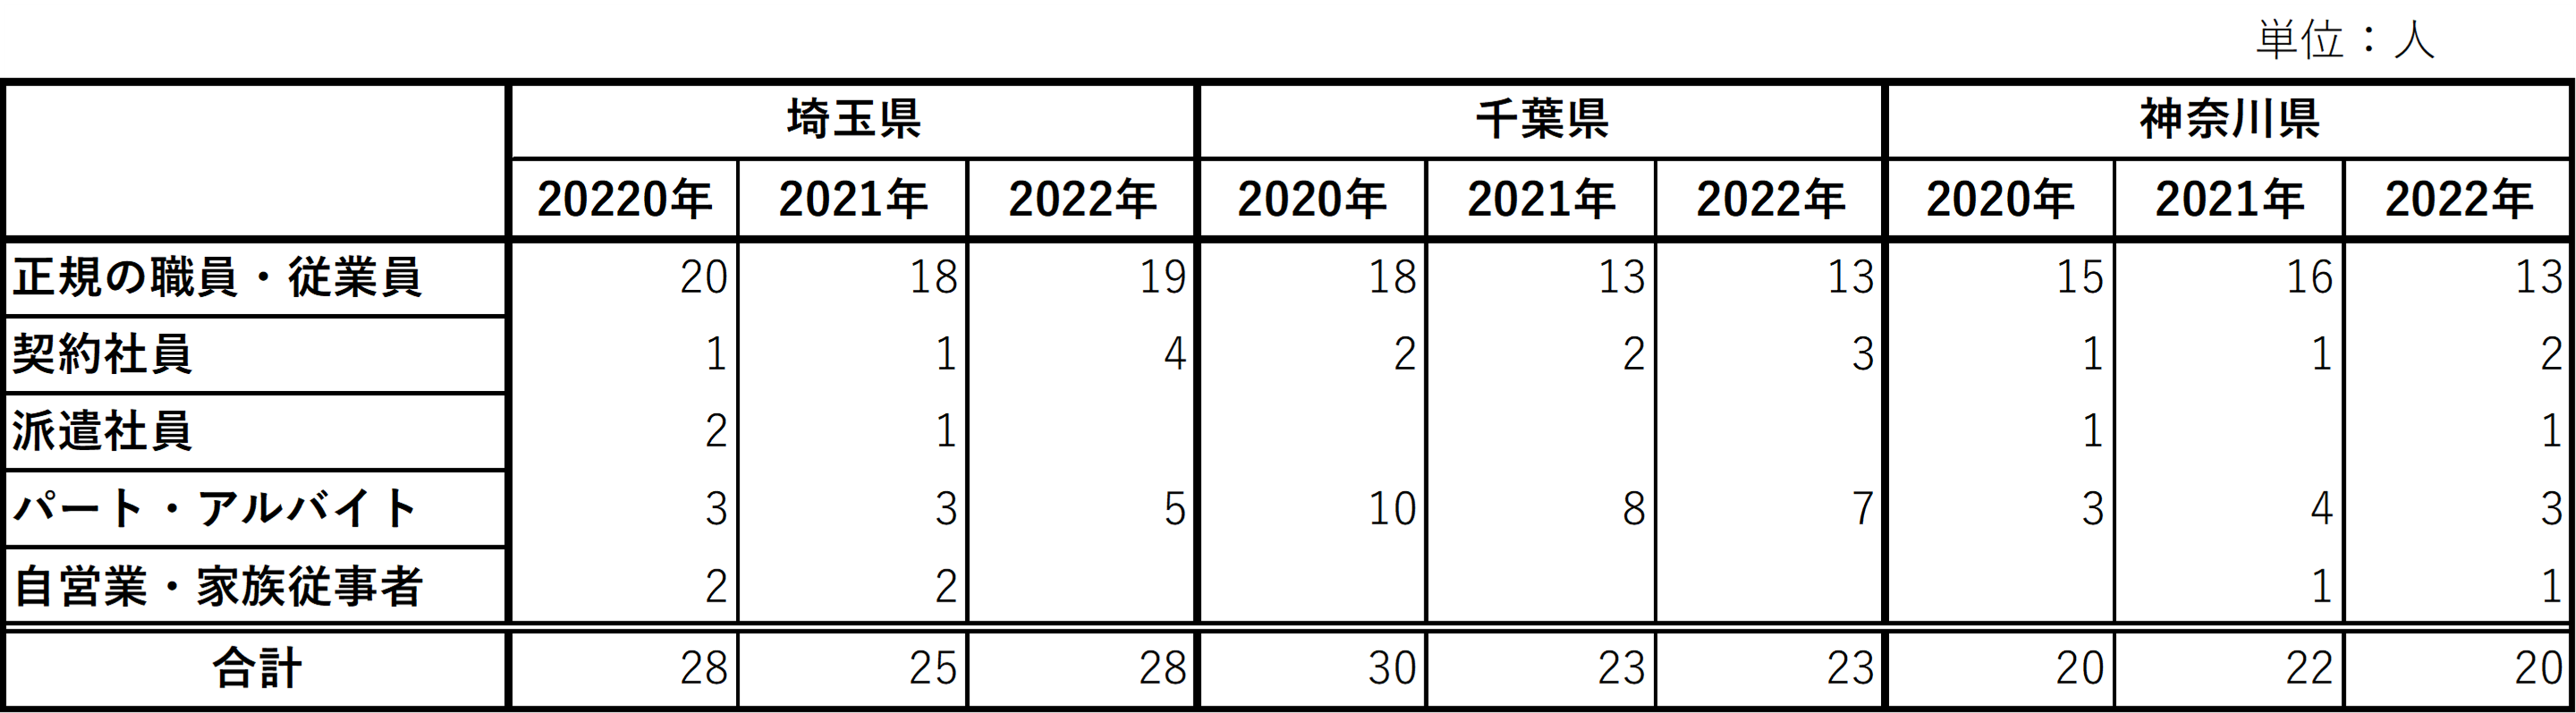
\includegraphics[width=110mm]{figure/c04s01_table_事務従事者_サンプル数.png}
  \label{sample_事務従事者}
\end{table}

どの地域でも正規の職員が10人以上いることが分かる。
また,図\ref{対象地域内における社会属性の人数と男女構成}を見ると,性別の偏りが少ないことが分かる。
そのため,国交省調査での事務従事者は,男女ともに正規雇用で従事している傾向にある。
そして,表\ref{生活活動-事務従事者}は,各調査日における事務従事者の過ごしていた場所,行った移動手段,行った活動の平均時間を表したものである。\\

\begin{table}[H]
  \centering
  \caption{コロナ禍における事務従事者の生活活動(単位:分)}
  \includegraphics[width=122mm]{figure/c04s01_table_事務従事者_生活活動.png}
  \label{生活活動-事務従事者}
\end{table}

% tableの平均時間の数値と増減幅の数値を区別してほしいという指摘と、"流行前から第1回緊急事態宣言下である2020年4月16日になると"の意味が分からないという指摘があった。\
流行前から2020年4月16日になると行動フラグ01自宅の時間が約200分以上増加している。
それと同時に,行動フラグ03勤務先の時間が相対的に減少している。
制限等が全て解除された後の2021年12月1日にかけて,自宅にいる時間は減少し,勤務先にいる時間が増加している。
その後,勤務先にいる時間は,まん延防止等重点措置下である2022年3月1日において緊急事態宣言下と同様に減少傾向にある。
BA5対策強化宣言後の2022年12月8日では,埼玉県と千葉県は増加傾向に転じている。
一方,神奈川県では平均301分から平均247分と約60分減少している。
2022年12月(未定日)は,在宅勤務を実施している者や実施していない者が混在しているため,勤務先にいる時間が減少している地域もあれば増加している地域もある。\\
 行動フラグ03勤務先と行動フラグ14仕事の関係を見ると,勤務先の時間が減ると仕事の時間も減る傾向にある。
例えば,流行前の千葉県は勤務先にいる時間が平均433分であり、仕事の時間が平均458分であった。
しかし,第1回緊急事態宣言下である2020年4月16日では勤務先にいる時間が平均154分であり、仕事の時間は平均397分となっている。
また,第1回緊急事態宣言解除後の2020年7月31日では,勤務先にいる時間は平均199分であり、仕事の時間は平均366分である。
そして,全ての制限が解除された直後の2021年12月1日には,勤務先にいる時間は平均382分であり、仕事の時間は平均550分であった。
このように,勤務先の時間と仕事の時間の増減には一定の関係が見られる。
そして,図\ref{時空間経路図_事務従事者}は,各調査日における事務従事者の時空間経路図である。\\

\begin{figure}[H]
  \centering
  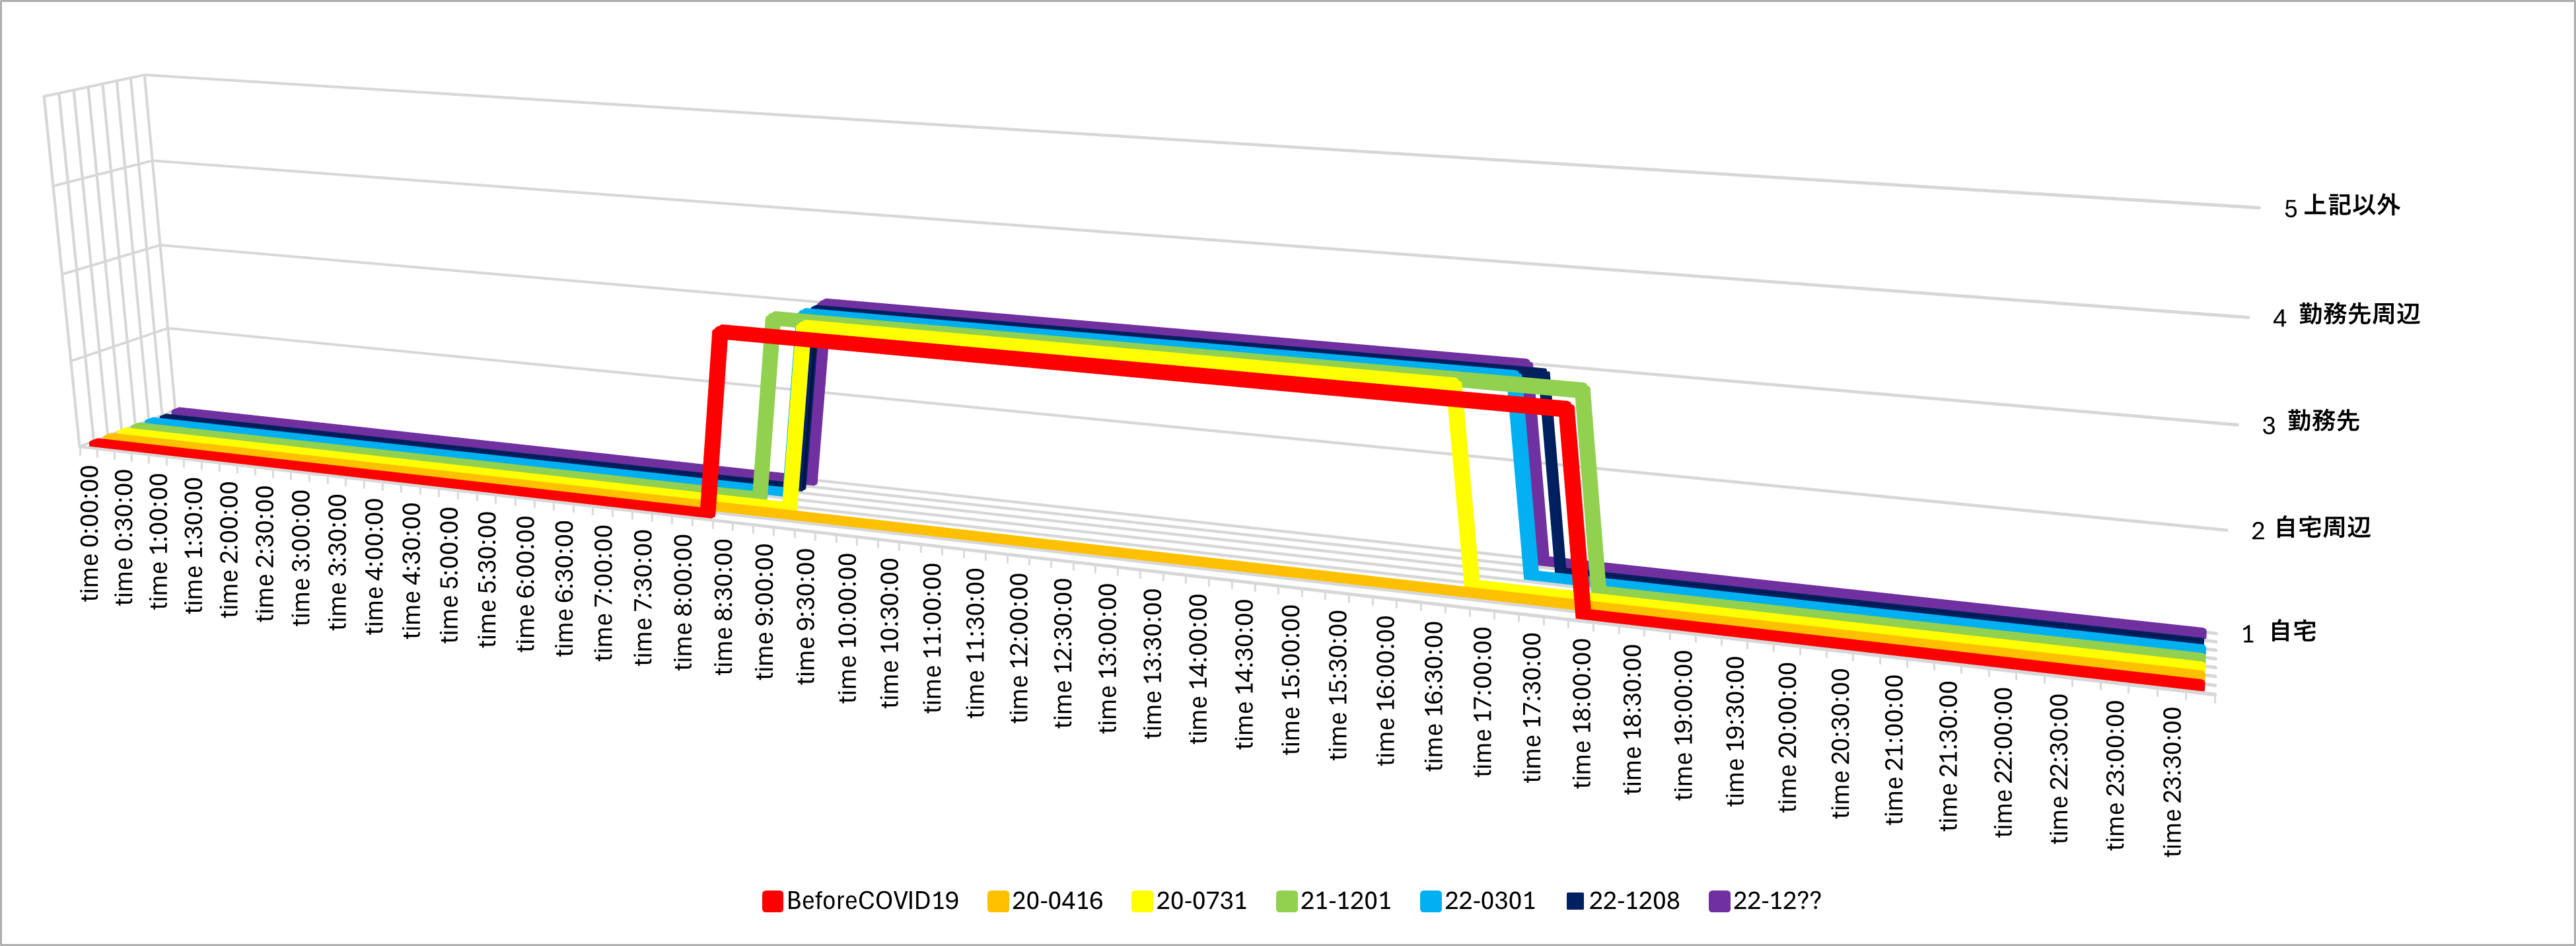
\includegraphics[scale=0.4]{figure/c04s01_fig_事務従事者_時空間経路図.png}
  \caption{事務従事者の時空間経路図}
  \label{時空間経路図_事務従事者}
\end{figure}

第1回緊急事態宣言下である2020年4月16日は,多くの事務従事者が自宅にいることが分かる。
表6では同日に7時間前後の仕事の時間があるため,多くが在宅勤務をしていたと考えられる。
また,勤務先での時間を見ると全面解除された2021年12月1日のみ流行前と同じような1日となっている。
それ以外の時点では,流行前よりも勤務先にいる時間が午前9時00分から午後17時00分までと短時間となっている。\\
 時空間の変容を見ると,おおよそ午前8時00分から午前9時30分までの間と午後17時00分から午後18時30分までの間の2つの時間帯で変動が起きている。
これらの時間帯は通勤時間帯と重なる。
それ故,コロナ禍における事務従事者の生活変容は通勤時間帯のタイミングで起こりやすいといえる。\\

\end{document}